\documentclass[12pt]{extarticle}

\usepackage{geometry}
\geometry{
a4paper,
total={170mm,257mm},
left=20mm,
top=20mm,
headheight=12pt
}

\usepackage[parfill]{parskip} % Activate to begin paragraphs with an empty line rather than an indent
\usepackage{graphicx}
\usepackage{amsmath, amssymb, amsthm}
\usepackage[font=small,labelfont=bf]{caption, subcaption}
\usepackage{setspace}\onehalfspacing
\usepackage[loose,nice]{units}
\usepackage{array}
\usepackage[super]{nth}
\usepackage{graphicx}
\usepackage{float}
\usepackage{varioref}
\usepackage[unicode=true,colorlinks=true,urlcolor=blue,citecolor=black,linkcolor=black]{hyperref}
\usepackage{cleveref}
\usepackage{subcaption}
\usepackage{mathtools}
\usepackage[all]{nowidow}
\usepackage{wrapfig}
\usepackage{pdfpages}
\usepackage{authblk}
\usepackage[utf8x]{inputenc}
\usepackage[english]{babel}
\usepackage{xcolor}
% appendix
\usepackage[title,page]{appendix}
\usepackage{chngcntr}
% unbreakable dashes
\usepackage[shortcuts]{extdash}
% footnotes
\renewcommand{\thefootnote}{\fnsymbol{footnote}}

% less space before sections 
% \titlespacing*{<command>}{<left>}{<before-sep>}{<after-sep>}
\usepackage{titlesec}
\titlespacing*{\section}
{0pt}{2ex plus 1ex minus .2ex}{2ex plus .2ex}
\titlespacing*{\subsection}
{0pt}{1ex plus 1ex minus .2ex}{1ex plus .2ex}
\titlespacing*{\paragraph}
{0pt}{1ex plus 1ex minus .2ex}{1ex plus .2ex}

%SetFonts
% newtxtext+newtxmath
\usepackage{newtxtext} %loads helv for ss, txtt for tt
\usepackage{amsmath}
\usepackage[bigdelims]{newtxmath}
\usepackage[T1]{fontenc}
\usepackage{textcomp}
%SetFonts

% Supplementary
% https://support.authorea.com/en-us/article/how-to-create-an-appendix-section-or-supplementary-information-1g25i5a/
\newcommand{\beginsupplement}{%
      	\setcounter{table}{0}
        \renewcommand{\thetable}{S\arabic{table}}%
        \setcounter{figure}{0}
        \renewcommand{\thefigure}{S\arabic{figure}}%
		\setcounter{equation}{0}
        \renewcommand{\theequation}{A\arabic{equation}}%
}
% NatBib
\usepackage[numbers,square,comma,sort]{natbib}
\renewcommand{\bibsection}{}
%\renewcommand{\bibfont}{\small}

% math stuff
\DeclareMathOperator*{\E}{{\rm I\kern-.3em E}}
\newcommand*{\tr}{^\intercal}
\let\vec\mathbf
\newcommand{\matrx}[1]{{\left[ \stackrel{}{#1}\right]}}
\newcommand{\diag}[1]{\mbox{diag}\matrx{#1}}
\newcommand{\goesto}{\rightarrow}
\newcommand{\dspfrac}[2]{\frac{\displaystyle #1}{\displaystyle #2} }
\newtheorem{theorem}{Theorem}
\newtheorem{corollary}{Corollary}
\newtheorem{lemma}{Lemma}
\newtheorem{remark}{Remark}
\newtheorem{result}{Result}
\renewcommand\qedsymbol{} % no square at end of proof
\newcommand{\cl}{\mathbf{L}}
\newcommand{\cj}{\mathbf{J}}
\newcommand{\ci}{I}

% line numbers
\usepackage[displaymath, mathlines]{lineno}
\renewcommand\linenumberfont{\normalfont\small\sffamily}
\linenumbers
\modulolinenumbers[2]


% Title page
\title{Prestige bias in cultural evolutionary dynamics}
% Authors
\renewcommand\Affilfont{\small}

\author[1,3]{Saar Egozi}
\author[2,3,$\dagger$]{Yoav Ram}

\affil[1]{School of Computer Science, Reichman University, Herzliya, Israel}
\affil[3]{School of Zoology, Faculty of Life Sciences, Tel Aviv University, Tel Aviv, Israel}
\affil[3]{Sagol School of Neuroscience, Tel Aviv University, Tel Aviv, Israel}
\affil[$\dagger$]{Corresponding author: yoav@yoavram.com}


\begin{document}
\maketitle

\begin{abstract}
{If the traits of more successful individuals are more likely to be adopted, the resulting cultural transmission is described as being success-biased. Prestige may be used as a proxy for successs.}
Here, we model prestige bias as a combination of indirect success bias and influence bias, the latter meaning that the choice of a role-model depends on the number of individuals that have already copied  that role-model.
{The} effect of prestige on cultural evolutionary dynamics {is analyzed} using mathematical analysis and stochastic simulations.
{Analytic} approximations to the stochastic role-model choice process {facilitate the} mathematical analysis and reduce the computational complexity of simulations. {Approximations are given}  to the fixation probability and the fixation time of an invading cultural trait in different environments. 
We show that indirect success bias effectively plays the role of natural selection, whereas influence bias effectively plays the role of genetic drift.	
Influence bias{, which may be strong in communities where social media are prevalent,}  also accelerates the evolutionary dynamics, as can be expected in a rich-{get}-richer process.
\end{abstract}


\pagebreak


\section*{Introduction}

%\paragraph{Cultural transmission.}
%In cultural transmission, individuals transmit cultural traits (i.e., behaviors, beliefs, norms) to one another, typically by learning and demonstrating \citep{transmissionVectorsBook}.
%Examples for cultural traits in humans are norms, preferences, tools, ideas, and language, potentially transmitted verbally and/or by observations \citep{transmissionVectors}. 
%Although cultural transmission is common in humans, it is also observed in other animals, e.g. chimpanzees \citep{chimpsPrestige, chimpsCopy}, dolphins and whales \citep{dolphins_whales}, elephants \citep{elepahntsRepo}, and even flies \citep{fliesPaper} and fish \citep{Truskanov2020}.

Cultural transmission {of attitudes, preferences, beliefs, norms, and behaviors} may combine vertical transmission, in which parents transmit to their offspring; oblique transmission, in which adults (teachers, leaders, and even strangers) transmit to unrelated offspring; and horizontal transmission, in which {individuals} from the same age cohort transmit to one another \citep{transmissionVectorsBook}.
It has been demonstrated that non-vertical cultural transmission can maintain maladaptive traits, which can be beneficial in changing environments \citep{changeEnv,Lehmann2009}. 

Transmission biases may cause a cultural trait to have a {higher rate of transmission than} its frequency in the population. \textit{Success bias} occurs when individuals prefer to copy from role models that demonstrate success in some activity, such as fishing, growing yams, using medicinal plants \citep{fijian_social_bias}, or hunting \citep{Mesoudi2008}, and it can increase the probability of learning a {trait that is present in those successful individuals} \citep{Borofsky2022}. 
Indeed, in a tournament between learning strategies  \citep{strategiesPaper}, most {winning} strategies included a mixture of success-biased social learning and individual learning, implying that success-biased learning is a good strategy, but that by itself it is not enough to best other strategies, even when success is measured accurately.

{Boyd and Richerson} \citep[Ch.~5]{evolutionBook} suggested that the {assessment} of success can be divided to three categories: \emph{direct bias}, \emph{indirect bias} and \emph{frequency-dependent bias}.
{Direct} bias occurs when one phenotype is more attractive than other phenotypes, and is evaluated by \emph{directly} testing the trait.
For example, an individual observing a ping-pong match can {try} the observed paddle grips to determine which grip is better.
Frequency-dependent bias occurs when the probability {of copying} a phenotype is higher or lower than the frequency of the phenotype among demonstrators. 
For example, suppose the common paddle grip is used by 60\% of the demonstrators; if the this grip is adopted by 80\% of copiers, then transmission is under positive frequency bias, also called \emph{conformity}; if it is adopted by 40\% of copiers, then transmission is under negative frequency bias, or \emph{{anti}-conformity} \citep{conformism}. 
The effects of conformity and {anti}-conformity on cultural evolution have been studied with both models \citep{anticonformity,Denton2021,conformity} and experiments \citep{negativeFrequency}.
Indirect bias occurs when an individual uses one phenotype to determine the attractiveness of another phenotype. % TODO change this to indirect evaluation instead of two phenotypes because we dont have two phenotypes
For example, an observer may copy the paddle grip of the {ping}-pong player who scored more points in the match, thus indirectly evaluating the grip by the points scored.
However, this may cause mismatches between the copied trait and the rest of the cultural or genetic repertoire of the individual \citep{Kolodny2022}.
Furthermore, {Boyd and Richerson} \citep[Ch. 8]{evolutionBook} {suggest} that maladaptive traits may spread widely in a population if indirect {bias is} strong enough, e.g., by a runaway process caused by a cultural equivalent of sexual selection \citep{sexualSelectionBook}.
Indeed, helping behaviors can evolve due to horizontal transmission bias even without any benefit to the recipient, or when the benefit is much larger than the cost \citep{cooperation}.

{Heinrich and Broesch \citep{fijian_social_bias}  studied} such indirect success biases, which they call cross-domain success bias or \emph{prestige bias} (e.g., great fishermen may be chosen as role-models for growing yams). They {suggested} that such biases, over generations, can lead to cultural adaptations, and that although prestige can lead to maladaptive traits spreading in the population, it can also accelerate the spread of adaptive traits
\citep[Ch.~8]{evolutionBook}. {Prestige bias may be} more common in humans than success {bias} \citep{complexityPaper}, and prestige is often mentioned in the cultural evolution literature, {although} there are few models of {it}.

A broader definition of prestige is the ``widespread respect and admiration felt for someone or something on the basis of a perception of their achievements or quality'' (New Oxford American Dictionary).
Indeed, Chudek et al.~\citep{prestige_cultural_learning} have defined prestige bias as ``a tendency to learn from individuals to whom others have preferentially attended, learned or deferred'', and demonstrated its occurrence in in 3-4 year old children.
{Henrich and Gil-White} \citep{prestige_evolution} gave a similar definition of prestige as ``freely conferred deference'', in contrast to \emph{dominance}, and provided examples from the anthropological literature.

To distinguish this form of indirect bias from other definitions of prestige, we call it \emph{influence bias}.
This is an important distinction, as influence is a context-dependent bias, rather than a content-{dependent} bias: it does not depend on the phenotype itself but rather on the number of copiers that have already copied each role-model, which may be easier and more accurate to estimate than success. 
Influence bias is also frequency independent (see \cref{cor:GBD} below), and thus it differs from conformity, which depend on the frequency of a trait in the population or in a sample of role-models, rather than the social dynamics of copying.

In contemporary human society, social media make it especially easy to estimate the social and cultural influence individuals have over others, which can have an effect on decision making. Online social networks such as \emph{Facebook} and \emph{Instagram} are known to affect the influence of individuals \citep{social_influence,social_media,influence_analysis}, and specific marketing practices have been invented to capitalize on this effect \citep{facebook_marketing}.

In the following, we develop a stochastic model of cultural transmission with prestige bias that combines both cross-domain indirect success bias and influence bias.
We develop analytic approximations for this model and analyze its dynamics. We also find approximations for the probability and time to fixation of a `successful' phenotype (i.e., that is {subject to} success bias). Comparing these approximations to Kimura's approximations for the fixation of a favorable allele \citep{kimura,kimura_average}, we demonstrate that success and influence bias play the role of natural selection and genetic drift, respectively. 

%%%%%%%%%%%%%%%%%%%%%%%%%%%%%%%%%%%%%%%%%%
\section*{Models}
% TODO explain indirect bias as indirect evaluation
We begin with a continuous trait model with indirect bias suggested by Boyd and Richerson~\citep{evolutionBook}, propose an extension with influence bias, and then develop a model with a dichotomous trait.
We implement our stochastic models and approximations, perform statistical analyses, and produce figures using Python \citep{python} with NumPy \citep{numpy} and Matplotlib \citep{mathplotlib}. 
Source code is available at \href{https://github.com/yoavram-lab/PrestigeBias}{https://github.com/yoavram-lab/PrestigeBias}.

\subsection*{Continuous trait}
We follow the Boyd and Richerson model~\citep{evolutionBook}, assuming only oblique transmission of a single trait. 
Consider a population of $N$ individuals, described by a single trait that takes continuous values.
Each generation, $N$ naive individuals, or copiers, each chooses a single role-model from the entire previous generation. The copier than copies its trait value from the chosen role-model.
Note that our transmission models is slightly different than previous those modeled before, e.g. \citep{cumul_culture,anticonformity,evolutionBook}, in which the population is infinite and each copier samples $n$ role-models and then copies its trait from one or more of the sampled role-models.

Similar to a Wright-Fisher model, generations are non-overlapping, and the entire population is replaced in each generation.
The population at time $t$ can be described by $\vec{A}(t)=\big(A_{1}(t), \ldots, A_{N}(t)\big)$ where $A_{i}(t)$ is trait value of individual $i$ at time $t$, and  the initial population is drawn from a standard normal distribution, $\vec{A}(0) \sim N(0,1)$ .
Cultural transmission is modeled by a function $F$ such that 
\begin{equation}\label{eq:transmission}
A_{i}(t+1) = F_i(\vec{A}(t)) \;.
\end{equation}

\paragraph{Success bias.}
Boyd and Richerson~\citep[Ch.~8, p.~247-249]{evolutionBook} describe a  transmission algorithm by defining $F$, a weighted average of the traits of all role-models, as
\begin{equation}\label{eq:boydF}
F_i(\vec{A}) = \sum_{j=1}^N G_{i,j}\cdot A_{i,j} \;, 
\end{equation}
where $G_{i,j}$ is the success bias of role-model $j$ in the eyes of copier $i$,
\begin{equation}\label{eq:boydG}
G_{i,j} = \frac{\beta(A_{i,j})}{\sum_{k=1}^{N} \beta(A_{i,k})} \;,
\end{equation}
$A_{i,j}$ is the absolute trait value {that} copier $i$ estimates for role-model $j$ with some error $e_i \sim N(0,\eta^2)$,
\begin{equation}\label{eq:relativeTrait}
A_{i,j} = A_j + e_i,
\end{equation}
and $\beta(\cdot)$ is the bias function that quantifies the success bias of a role-model \citep[eq.~5.11]{evolutionBook},
\begin{equation}\label{eq:success_bias}
\beta(A_{i,j}) = b \cdot \exp{\Big(-\frac{(A_{i,j} - \hat{A})^2}{2J}\Big)} \;,
\end{equation} 
with $\hat{A}$ as the arbitrary optimal trait value, and $J$ and $b$ as parameters that control the bias strength.
Therefore, $G_{i,j}$ is a relative success score that copier $i$ assigns to role-model $j$.

Boyd and Richerson~\citep{evolutionBook} note that the deterministic blended transmission algorithm they use has alternatives. We {can} develop a similar stochastic model with transmission from a single random role-model where instead of \cref{eq:boydF}, we define the transmission function $F$ as a random variable with its distribution given by 
\begin{equation}\label{eq:ourF}
\Pr\big(F_i(\vec{A}) = A_{j}\big) = G_{i,j} \;;
\end{equation}
{here $G_{i,j}$ is} the probability {that copier $i$ chooses} to copy the trait of role-model $j$.

\paragraph{Influence bias.}
Here we introduce a new element to the model by assuming that in each generation, copiers choose their role-models one by one.
{Denote by} $K_{i,j}$  the number of copiers that {choose} role-model $j$ after copier $i$ chose a role-model. Thus, $i$ out of $N$ copiers {had} already {chosen} a role-model, $\sum_{j=1}^N{K_{i,j}} = i$, and there are $N-i$ copiers that have yet to choose a role-model.
The stochastic process of role-model choice, 
\begin{equation} \label{eq:process}
\big\{\vec{K}_i = (K_{i,1}, \ldots, K_{i,N}) \big\}_{i=1}^N \;,
\end{equation}
is described by the recurrence equation
\begin{equation} \label{eq:recurrence}
K_{i,j} = K_{i-1,j} + S_{i,j}, \quad i,j=1,2,\ldots,N \;,
\end{equation}
where $S_{i,j}=1$ if the $i$-th copier chose role-model~$j$ and 0 otherwise, and the initial state is $K_{0,j}=0$.

Following \cref{eq:ourF}, the probability that the $i$-th copier chose role-model $j$ is given by the prestige of role-model $j$ in the eyes of copier $i$,
\begin{equation}\label{eq:recPrestige}
Pr(S_{i,j}=1 \mid S_{1,j},S_{2,j},...,S_{i-1,j}) = G_{i,j} \;.
\end{equation}
The prestige $G_{i,j}$ of role-model~$j$ in the eyes of copier~$i$ is determined by success--the estimated biased trait value $\beta(A_{i,j})$--and influence--the number of copiers that chose role-model $j$ before copier $i$, $K_{i-1,j}$, replacing \cref{eq:boydG} with
\begin{equation}\label{eq:prestige}
G_{i,j} = \frac{\alpha_{ij} \cdot \beta(A_{i,j}) + (1-\alpha_{ij}) \cdot K_{i-1,j}}{W_i} \;,
\end{equation}
where $W_i$ is a normalizing factor that sums the numerator over all role-models ($1\le j \le N)$ to ensure $\sum_{j=1}^{N}{G_{i,j}}=1$.

Here, the bias weight $\alpha_{i,j}$ determines the relative weighting of success and influence bias. It is a characteristic of the interaction of role-model~$j$ with copier $i$ that determines the relative significance of direct success vs. influence in the role-model's overall prestige in the eyes of the copier.
Different individuals may evaluate the importance of success and influence differently. Additionally, we assume each role-model displays its influence and success individually. For example, individuals with more followers but lacking skill may emphasize the number of their followers rather than their skill.
Finally, the trait of role-model $j$ estimated by copier $i$, $A_{i,j}$, remains as in \cref{eq:relativeTrait}.



\subsection*{Dichotomous trait}
{We} introduce a simplified version where the trait {has only} two phenotypes: {an} optimal phenotype $\hat{A}$ and {a} sub-optimal phenotype $A$. 
All role-models with the same phenotype will contribute to the probability {that} that phenotype {is} transmitted, and thus influence is determined by the number of copiers that have already chosen a role-model with either phenotype.
In addition, for simplicity and for easier mathematical analysis, we assume $\alpha$ is homogeneous, {which entails} exchangeability between role-models.
Therefore, the probability {that} the $i$-th copier {copies} phenotype $A$ is
\begin{equation}\label{eq:binary-model}
G_{i,A} = \frac{(N-X)\alpha'\beta(A) + K_{i,A}}{i-1 + (N-X)\alpha'\beta(A) + \alpha'X} \;,
\end{equation}
where $X$ is the number of role-models with trait $\hat{A}$; $K_{i,A}$ is the number of copiers that already chose $A$ when copier $i$ chooses a role-model; assuming (without loss of generality) that $\beta(\hat{A})=1$; and defining $\alpha'= \frac{\alpha}{1-\alpha}$ as the odds ratio of the bias weight.
Complementing this, the probability of the $i$-th copier to copy phenotype $\hat{A}$ is $G_{i, \hat{A}} = 1-G_{i,A}$.
The rest of the details follow the continuous trait model.


%%%%%%%%%%%%%%%%%%%%%%%%%%%%%%%%%%%
\section*{Results}
Our models are defined by two nested stochastic processes. Change over multiple generations is described by the {dynamics of the} phenotype distribution at each generation, $\{\vec{A}(t)\}_t$, see \cref{eq:transmission}. The transition from one generation to the next is described by the number of copiers each role-model has after $i$ copiers have chosen a role-model, $\{\vec{K}_i\}_{i=1}^N$, see \cref{eq:process}.
We emphasize that the models are nested: $\vec{A}(t+1)$ can be computed from $\vec{A}(t)$ by evaluating $\vec{K}_{N}$, where $K_{N,j}$ is the number of copiers that chose role-model $j$ after all copiers chose a role model.
However, the former requires iterating over \cref{eq:recurrence,eq:recPrestige}.
Thus, we sought to find an equivalent stochastic process that has the same joint distribution as $\vec{K}_{N}$. 
We found two approximations for the distribution of $\vec{K}_{N}$, summarized here and explained in detail below.
In both we assume that the bias weight is either completely homogeneous, $\alpha_{i,j}=\alpha$, or that $\alpha_{i,j}=\alpha_j$ is a bias of role-model $j$ only, meaning it does not vary between copiers. %TODO but result 1 has alpha_i
Note that these approximations apply for both the and the continuous trait (\cref{eq:prestige}) and the dichotomous trait (\cref{eq:binary-model}) models.

\paragraph{Generalized binomial approximation.}  
The number of copiers of a specific role-model at each step, $K_{i,j}$, follows the {\em generalized binomial distribution}~\citep{GBD} and therefore,


(i) the expected number of copiers of role-model~$j$ equals its prestige in the eyes of the first copier, multiplied by the total number of copiers, that is,
$\E[K_{N,j}] = N \cdot G_{1,j}$ if trait estimation error is uniform for all copiers ($e=e_i$ for $i=1, \ldots, N$); and
(ii) the expected number of copiers of each role-model equals its relative biased trait value, similar to the role of relative fitness in population-genetic models, that is, $\E[K_{N,j}] = \beta(A_j+e) / \overline{\beta}$ if the bias weight is uniform for all role-models ($\alpha=\alpha_j$ for $j=1,\ldots,N$), where $\overline{\beta}=1/N \sum_{j=1}^{N}{\beta(A_j+e)}$ is the population mean estimated trait value. 

\paragraph{Dirichlet-Multinomial approximation.}
The role-model choice process, $\{\vec{K}_{i}\}_{i=1}^{N}$, is equivalent to a {\em P\'{o}lya urn} model if trait estimation error is uniform for all copiers ($e=e_i$ for all $i=1, \ldots, N$), meaning that the order of copiers does not matter. 

\subsection*{Generalized binomial distribution}
The generalized binomial distribution (GBD) emerges from a series of dependent Bernoulli trials (in contrast to the standard binomial distribution in which trials are independent) and is {denoted}  by $GBD(n, p, \theta)$ where $n$ is the number of trials, $p$ is the probability of success of the first trial, and $\theta$ is the correlation between trials ($\theta=0$ gives the standard binomial distribution).
\\

\begin{result}[Generalized binomial approximation]\label{res:GBD}
The number of copiers of role-model $j$ after $i$ copiers have chosen a role-model follows the GBD, $K_{i,j} \sim GBD(i,\alpha_i\cdot\beta(A_j+e))$ if $e_i=e$ for all role-models $i=1, \ldots, N$. % TODO what about theta?
\end{result}

\begin{proof}
{Let} $Q_j(k,i)=P(K_{i,j} = k \mid K_{i-1,j})$ {be} the probability that exactly $k$ out of $i$ copiers choose role-model $j$ given $K_{i-1,j}$ {out} of $i-1$ copiers chose role-model $j$. 
Using conditional probability and \cref{eq:recurrence},
\begin{equation}\label{recursive}
Q_j(k,i) = P_j(S_{i,j}=1 | k-1,i-1) \cdot Q_j(k-1,i-1) + P_j(S_{i,j} =0 | k,i-1) \cdot Q_j(k,i-1) \;,
\end{equation}
where $S_{i,j} =1 $ when the $i$-th copier chooses role-model $j$.
\Cref{recursive} is equivalent to eq.~(2.1) in \citep{GBD}, which completes the proof.
\end{proof}

This result gives the following corollary on the expected number of followers of a given role-model $j$ by the end of the role-model choice process, $K_{N,j}$.
\\


\begin{corollary}\label{cor:GBD} The expected number of copiers of role-model $j$ after all copiers have chosen a role-model is
$\E[K_{N,j}] = N \cdot G_{1,j}$, where $G_{1,j}$ is the probability of the first copier to copy role-model $j$.
In addition, $\E[K_{N, j}] = \alpha_j \cdot \beta(A_j+e) / \overline{\alpha \cdot \beta(A+e)}$, where the averaging in the denominator is over the role-models index, $j$.
\end{corollary}

\begin{proof}
Drezner and Farnum~\citep[eq.~(2.3)]{GBD} show that the expected number of successful trials, 
$\E[k] = N \cdot Q_j(1,1)$ (modified from their notation). %TODO what is k? not defined.
Here, $Q_j(1,1)$ is the initial probability to choose role-model $j$, before any role-model choices are made.
$Q_j(1,1) = G_{1,j}$ by definition.
The rest of the proof is in Appendix~\ref{sec:GBD}.
\end{proof}

%% TODO two sentences - influence bias is not frequency dependent

The special case where the bias weight is uniform for all role-models ($\alpha = \alpha_j$ for $j=1,\ldots, N$) is interesting, because we can evaluate the expected number of copiers using a linear equation
\begin{equation}\label{eq:GBDsamelalpha}
\E[K_{N,j}]= N\cdot\frac{\alpha\cdot\beta(A_j+e)}{\sum\limits_{m=1}^{N}\alpha\cdot\beta(A_m+e)} =\beta(A_j+e) \bigg/ \overline{\beta(A+e)} \;,
\end{equation}
where the only variable is $A_j+e$, because $\overline{\beta(A+e)}$ is the mean of the distribution of the trait values, modified by some constant parameters of $\beta$.
We can then write $L = 1/\overline{\beta(A+e)}$ and
\begin{equation}\label{eq:linearEq}
\E[K_{N,j}] = L\cdot \beta(A_j+e) \;.
\end{equation}

\paragraph{Numerical validation.}
To validate that GBD approximation for the number of copiers of a role-model is correct (\cref{eq:GBDsamelalpha}), %TODO check that this is the correct equation reference
we ran $1,000$ simulations of the full model, and compared the results with \Cref{cor:GBD}.
We compare the distribution of number of copiers by plotting the histograms of both our simulations results and the expected values based on \Cref{cor:GBD}.

Although basic, \Cref{fig:GBD} shows good fit of the GB approximation.
This validation is initial, and {we do} more extensive validations on the Dirichlet-Multinomial approximation, because {that} is what we will use in our {analysis}.

%%%%%%%%%%%%%%%%%%%%%%%%%%%%%%%%%%%
\subsection*{Dirichlet-Multinomial distribution approximation}

\paragraph{P\'{o}lya urn model.}
This stochastic process consists of $N$ draws from an urn with an initial {number} of colored balls of $M$ colors. When a ball is drawn, it is then placed back in the urn together with an additional new ball of the same color.
Let $\vec{U_i} = \{u_{i,1},u_{i,2},...,u_{i,M}\}$  where $u_{i,j}$ is the number of balls of the $j$-th color in the urn after $i$ draws.
Let $S_{i,j}=1$ when drawing a $j$-colored ball on the $i$-th draw, and $0$ otherwise. The probability that $S_{i,j}=1$ given $\vec{U_{i-1}}$ is
\begin{equation}\label{eq:polya}
\begin{split}
P(S_{i,j} = 1 \mid \vec{U_{i-1}}) = 
\frac{u_{i-1,j}}{\sum\limits_{m=1}^{M} u_{i-1,m}} = 
\frac{o_j + w_{i-1,j}}{\sum\limits_{m=1}^{M} o_m + w_{i-1,m}} = 
\frac{o_j + w_{i-1,j}}{i-1 + \sum\limits_{m=1}^{M} o_m} \;,
\end{split}
\end{equation}
where $o_j$ is the initial number of balls of color $j$ in the urn, and $w_{i,j}$ is the cumulative number of new balls that were added to the urn after $i$ draws of color $j$.
\\

\begin{result}[P{\'{o}}lya urn model]\label{result:polya}
The role-model choice process, $\big\{\vec{K}_i\big\}_{i=1}^N$, is equivalent to a \emph{P\'{o}lya urn model} if both trait estimation error and bias weight are uniform in the population, $e=e_j$ and $\alpha=\alpha_j$ for all $j=1,\ldots,N$.
\end{result}

\begin{proof} 
{Write} $\alpha'=\frac{\alpha}{1-\alpha}$ as the bias weight ratio, and $A'_j=A_j+e$. From \cref{eq:prestige} and because $\sum_{j=1}^{N}{K_{i,j}}=i$, we have
\begin{equation}\label{eq:copier_choose}
G_{i,j} = 
\frac{\alpha'\beta(A'_j) + K_{i-1,j}}{\sum\limits_{m=1}^{N}{\left[ \alpha'\beta(A'_m) + K_{i-1,m}\right]}}
 =\frac{\alpha'\beta(A'_j) + K_{i-1,j}}{i-1 + \sum\limits_{m=1}^{N}\alpha'\beta(A'_m)} \;.
\end{equation}
Substituting $M=N$, $o_j = \alpha'\beta(A'_j)$, and $w_{i,j} = K_{i,j}$ in \cref{eq:polya} gives \cref{eq:copier_choose}, thus completing the proof.
\end{proof} 

Frigyik et al.~\citep[section 2]{dirichlet} prove that the proportion of different colored balls in a \emph{P\'{o}lya urn model} converges to the Dirichlet distribution as the number of draws  (the population size, $N$, in our model) approaches infinity, based on the \emph{Martingale Convergence Theorem} \citep{martingaleBook}.
We therefore have an approximation for the relative prestige each role-model has when evaluated by copiers. Thus, choosing the role-models for all copiers is equivalent to drawing from a {multinomial} distribution where the parameters are the modified weights from a Dirichlet distribution and we have the following corollary.
\\

\begin{corollary}\label{cor:dirichlet}
The number of copiers of each role-model {approximates} a Dirichlet-Multinomial distribution, $\vec{K_i} \sim \emph{DM}(N,\vec{G_1})$, under the conditions of \Cref{result:polya}.
\end{corollary}

\paragraph{Numerical validation.}
% TODO add something about small N
We next validated the DM approximation of our model
and tested its sensitivity to the assumptions ($e_i=e$ and $\alpha_i=\alpha$ for $i=1,\ldots,N$) by comparing results of stochastic simulations of our model (\cref{eq:binary-model}) with the DM approximation (\Cref{cor:dirichlet}).
First, we computed an observed distribution of the number of copiers from the average empirical distribution of multiple simulations.
We then compared this observed distribution with the expected theoretical DM distribution (\Cref{fig:DM_validation}A).
The difference in distributions was not perceived when plotting both distributions on the same figure, so we used the difference instead.
The maximum difference is 0.5 role-models, which indicates a very good fit.
In addition, we tested the likelihood of the observed data to be drawn from the DM distribution, against a shuffle of the parameters vector of the DM distribution itself (\Cref{fig:DM_validation}B). We see that the negative log likelihood of the observed data is much higher than any other shuffled version of the parameters vector, strongly supporting our approximation.

Next, we examined the fixation probability and fixation time of a favored phenotype $\hat{A}$ when invading a population of phenotype $A$ and compared results from the full model and the DM approximation.
Thus, we assume the population has a single individual with phenotype $\hat{A}$ and $N-1$ individuals with phenotype $A$. 
That the number of simulations needed to sufficiently approximate our model with the DM approximation is roughly $1,000$ (\Cref{fig:num_sims}).
We examined the robustness of the DM approximation to relaxing the following assumptions.
First, we relaxed our assumption of no estimation error $e$.
Estimation error in the original model was drawn from a normal distribution, and added to the trait value before evaluation of the bias ($A_{i,j} = A_j + e_i$).
When estimation error is applied, we sample $J_i$ for each copier $i$ from a normal distribution with expected value zero and variance $\eta^2$. % TODO should e_i?
Even when the estimation error variance is $0.1$, both the fixation probability and fixation time approximations are accurate~(\Cref{fig:hetro_error}). 
We also relaxed our assumption of a uniform bias weight $\alpha$ (i.e., $\alpha_i=\alpha$). We allowed $\alpha$ to vary in the population, drawing $\alpha_j$ for each role-model $j$ from a normal distribution such that $\alpha_j \sim N(0.5,q)$ where $\epsilon$ is between $10^{-7}$ and $10^{-1}$. 
We found again that results of the DM approximation are similar to those from stochastic simulations of the full model~(\Cref{fig:hetro_alpha}).


%%%%%%%%%%%%%%%%%%%%%%%%%%%%%%%%%%%%%%%%%%%
\subsection*{Fixation probability and time}
After finding that the DM distribution is a good approximation of the (within-generation) role-model choice process, we turn our attention to the (between-generation) evolutionary dynamics.
We focus on the fixation probability and conditional fixation time (conditioned on the population reaching fixation) of a favored phenotype, using a diffusion-equation approximation approach, similar to analyses of population-genetic models \citep{kimura,kimura_average,otto_fixation}.
We are mainly interested in the effect of the bias weight, $\alpha$, which determines the relative effect of success and influence on prestige bias, given by \cref{eq:prestige}.
For simplicity, we use the dichotomous model, and we do not include role-model estimation error in this analysis, i.e $e_i=0$ for every copier $i$.
As shown above, transmission in our model is approximately DM distributed (\Cref{cor:dirichlet} and \cref{eq:copier_choose}).

\paragraph{Drift and diffusion terms in a constant environment.}
We start by finding the expectation and variance of the change in frequency from one generation to the next, which are the drift and diffusion terms of the diffusion equation.
Let $x$ and $x'$ be the frequency of type $\hat{A}$ in a population with $N$ individuals in the current and next generation, and  $\beta$ be the success coefficient of phenotype $A$, $\beta = \beta(A) < \beta(\hat{A}) = 1$.
% TODO can we say beta=beta(A)/beta(hat A) ? because beta(A hat)=b and not 1.
Then (see Appendix~\ref{sec:drift_diff_const} for derivation),
\begin{equation}\begin{aligned}
E[x'-x] &= (x(1-x)(1-\beta) + o(1-\beta)  \;, 
\\
V(x'-x) &= x(1-x)\left(\frac{1}{\alpha N + (1-\alpha)}\right) + o\left(\frac{1}{\alpha N + (1-\alpha)}\right) \;.
\end{aligned}\end{equation} 

This analysis gives a surprising result relating the parameters $\alpha$ and $\beta$ to parameters of the classical Wright-Fisher model from population genetics:
the selection coefficient $s$, a measure of the effect of natural selection on the change in frequency of genotypes, and the effective population size, $N_e$, a measure of the effect of random genetic drift on the change in frequency of genotypes. 
In a diffusion-equation approximation of the classical Wright-Fisher model, the expectation and variance of the change in frequency are $E[x'-x]=x+x(1-x)s+o(s)$ and $V[x'-x]=x(1-x)/N_e$ \citep[eq.~7]{kimura}{, respectively}. 
Therefore, we have the following result.\\

\begin{result}[Effective selection coefficient and population size]\label{res:selection_coef}
The effective selection coefficient $s$ and effective population size $N_e$ can be written in terms of the success coefficient $\beta$ (\cref{eq:success_bias}), the bias weight $\alpha$ (\cref{eq:prestige}), and the population size $N$ as 
\begin{equation}
s=1-\beta, \quad N_e=\alpha N + (1-\alpha) \;.
\end{equation}
\end{result}

Note that when $N>>1$, $N_e \approx \alpha N$, resulting in a very convenient expression.\\

Using our effective selection coefficient, $1-\beta$, and effective population size, $N_e$, with the population-genetics fixation probability approximation given by \citep[eq.~8]{kimura}, we {obtain}:
\begin{result}[Fixation probability]
The fixation probability is approximately
\begin{equation}\label{eq:kimura_p}
\pi(x) = \frac{1-e^{-2(1-\beta)N_e x}}{1-e^{-2(1-\beta)N_e}},
\end{equation}
where $x$ is the initial frequency of the favored phenotype $\hat{A}$.
\end{result}

Similarly, we can use $1-\beta$ and $N_e$ in the population-genetics fixation time approximation given by \citep[eq.~17]{kimura_average}.\\

\begin{result}[Fixation time] The expected fixation time (conditioned on fixation) from an initial frequency $x$ is approximately
\begin{equation} \label{eq:kimura_t}
T(x) = J_1(x) + \frac{1-\pi(x)}{\pi(x)}\cdot J_2(x),
\end{equation}
where $N_e=\alpha N + (1-\alpha)$, $S=N_e(1-\beta)$, and
\begin{equation}
\begin{aligned}
J_1(x) &= \frac{-1}{(1-\beta)(e^{-2S}-1)}\int_x^1 \frac{1-e^{2S\xi}-e^{-2S(1-\xi)}+e^{-2S}}{\xi(1-\xi)}d\xi \;, \\
J_2(x) &= \frac{-1}{(1-\beta)(e^{-2S}-1)}\int_0^x \frac{(1-e^{2S\xi})(e^{-2S\xi}-1)}{\xi(1-\xi)}d\xi \;.
\end{aligned}
\end{equation}
\end{result}
Note that these integrals cannot be solved in closed form, {and are estimated} numerically.

\paragraph{Numerical validation.}
We compare our approximations (\cref{eq:kimura_p,eq:kimura_t}) with results of simulations of our dichotomous model using various $\alpha$ and $\beta$ values, as well as simulations of the Wright-Fisher model, using the effective selection coefficient, $1-\beta$, and effective population size, $N_e=\alpha N + (1-\alpha)$. 
We find see that the two models have similar dynamics, and both are well approximated {by} our approximations (\Cref{fig:var_alpha}).


\begin{figure}[h]
    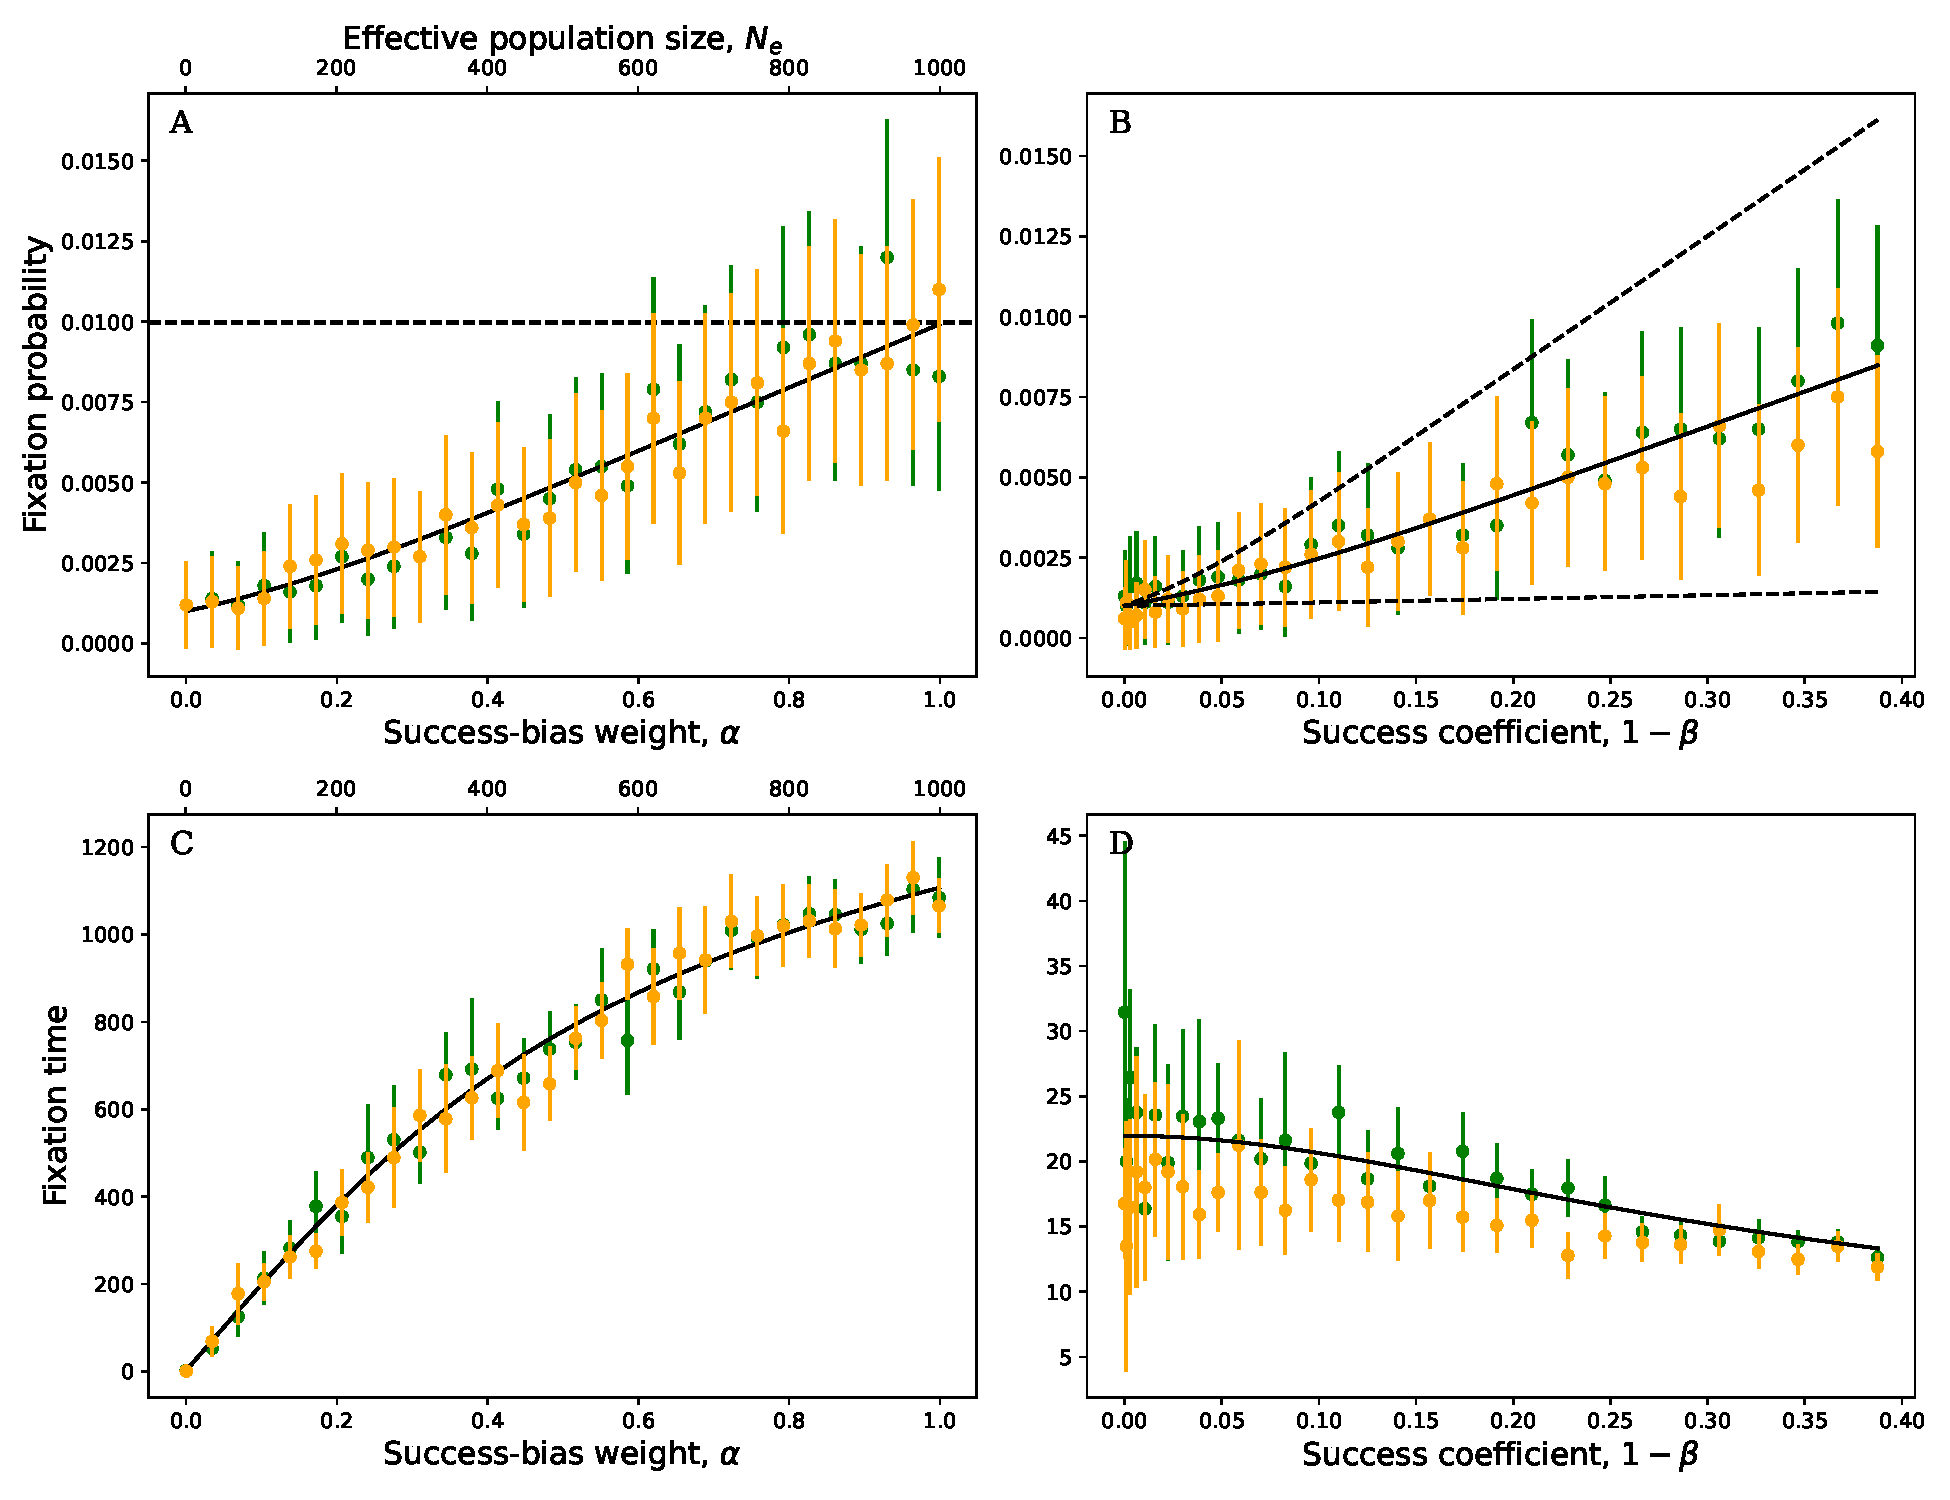
\includegraphics[width=\linewidth]{kimura_var.pdf}
  \caption{\textbf{Fixation probability and time in a constant environment.}
  Fixation probability and time (in generations) as a function of the success-bias weight $\alpha$ (bottom x-axis), or effective population size $N_e$ (top x-axis) in the top row, and as a function of the success coefficient, $1-\beta$, on the bottom row.
  The approximation (black; \cref{eq:kimura_p}) agrees with both DM simulations (green) and Wright-Fisher simulation (orange).
  Fixation probability (A) is bounded by $2(1-\beta)$ (blue).
  Markers are averages of $10,000$ simulations, error bars show 95\% confidence intervals for panels A and B and 75\% for panels C and D.
   Here, Population size, $N=1,000$; phenotype values, $A=0.7$ (panels A and B), 
   $A/\hat{A}$ is between 0.01 and 0.99 (panels C and D), and $\hat{A}=1$; % TODO not clear, because x label suggest you modify beta, but caption says you modify A/hatA. remind us that beta is given from A - refer to equation
   success coefficient, $1-\beta=s=0.044$ (panels A and B); 
   success-bias weight, $\alpha=0.01$ (panels C and D).
   }
  \label{fig:var_alpha}
\end{figure}


\paragraph*{Changing environment}. After finding a good approximation in a constant environment, where the favorable trait is always $\hat{A}$, we proceeded to find an approximation for when the environment changes. 
Following \citep{changeEnv}, we denote $k$ as the number of generations in which the invading phenotype is favored by success bias, and $l$ as the number of generations in which the resident phenotype is favored by success bias.
We then proceed to find expressions for the expectation and variance of the change in frequency between $n=k+l$ generations. 
The proof is in Appendix~\ref{sec:drift_diff_chang}.
\\

% TODO same as above, the derivation of drift and diffusion doesnt have to be a result of its own, but rather the fixation prob can be a result
\begin{result} [Drift and diffusion terms in a changing environment]\label{res:ch_expected}
Let $x$ be the initial frequency of the invading phenotype and $X_t$ the number of individuals with that phenotype after $n$ generation.
Then,
\begin{equation}\label{eq:ch_expected_and_var}
E[X_n/N - x] \simeq x(1-x) S_n / N_e \;, 
\quad
\text{and}
\quad
V(X_n/N-x) \simeq  n x(1-x) / N_e \;,
\end{equation}
where $S_n=\sum\limits_{t=1}^{n} N (1-\beta_t)$ and $\beta_t$ is $\beta(A)$ at generation $t$. % TODO define more explicitly how environmental change affects A and beta. define it before the result!
\end{result}

Note that here, we have the average selection coefficient during a cycle of $n$ generations as the selection coefficient {in} \cref{eq:kimura_p}.
Using the drift and diffusion terms and following \citep{changeEnv}, we can approximate the fixation probability in a changing environment using
\begin{equation}\label{eq:ch_env}
\tilde\pi(x) = \frac{1-e^{-2 \frac{S_n}{n} N_e x}}{1-e^{-2 \frac{S_n}{n} N_e}} \;.
\end{equation}

\paragraph{Numerical validation.}
To validate the the approximation for the fixation probability in a changing environment (\cref{eq:ch_env}), we compare it to results of simulations that use the DM approximation (\Cref{cor:dirichlet}).
We find that the approximation fits the simulation results well for variable bias weights, $\alpha$, which corresponds to the effective population size (\Cref{fig:ch_env_alpha_beta}A).

However, the approximation is more sensitive to the value of the success bias coefficient $\beta$ (\Cref{fig:ch_env_alpha_beta}B).
We suspect that when $\beta$ is too small, there will not be many cycles in the simulations, because either the population reaches a high frequency of the fitter phenotype after just a few cycles, or the fitter phenotype {goes} extinct very quickly. 
For such $\beta$ values (below 0.65), the fixation probability exceeds even the constant environment approximation (which is the upper limit). We note that the diffusion-equation approximation assumes weak selection, or in our case, weak success bias.

We found that for a large $k/l$ ratio (with a constant cycle length, $n=k+l=100$), the changing environment approximation (\cref{eq:ch_env}) converges to the constant environment approximation (\cref{eq:kimura_p}), see \Cref{fig:ch_env_alpha_beta}C and \Cref{fig:ch_env_alpha_beta}D.

The approximation follows the trend of the simulation results for all $\alpha$ values.
{On} increasing the success coefficient {$\alpha$} to more than 0.15, the simulation results were located above the changing environment approximation, and below the constant environment approximation. We believe the reason is the structure of the cycle.
Our proof and approximation in the changing environment are for a large {number} of cycles, and when the success coefficient {$\alpha$} is too high, there might be very few cycles. Either the ideal trait is copied by enough copiers so that the influence is sufficient to negate the success bias when the cycle changes (and the trait favored by the bias becomes the disfavored), or the opposite happens, and the ideal trait {goes} extinct before there {are} enough copiers that copied it.
We then tried to change the ratio between the number of cycles where $\hat{A}$ is favored and disfavored. We showed that the approximation fits well regardless of the ratio, but when the ratio of favored generations to disfavored ones is very high, it is very similar to a constant environment model.



\begin{figure}[H]
    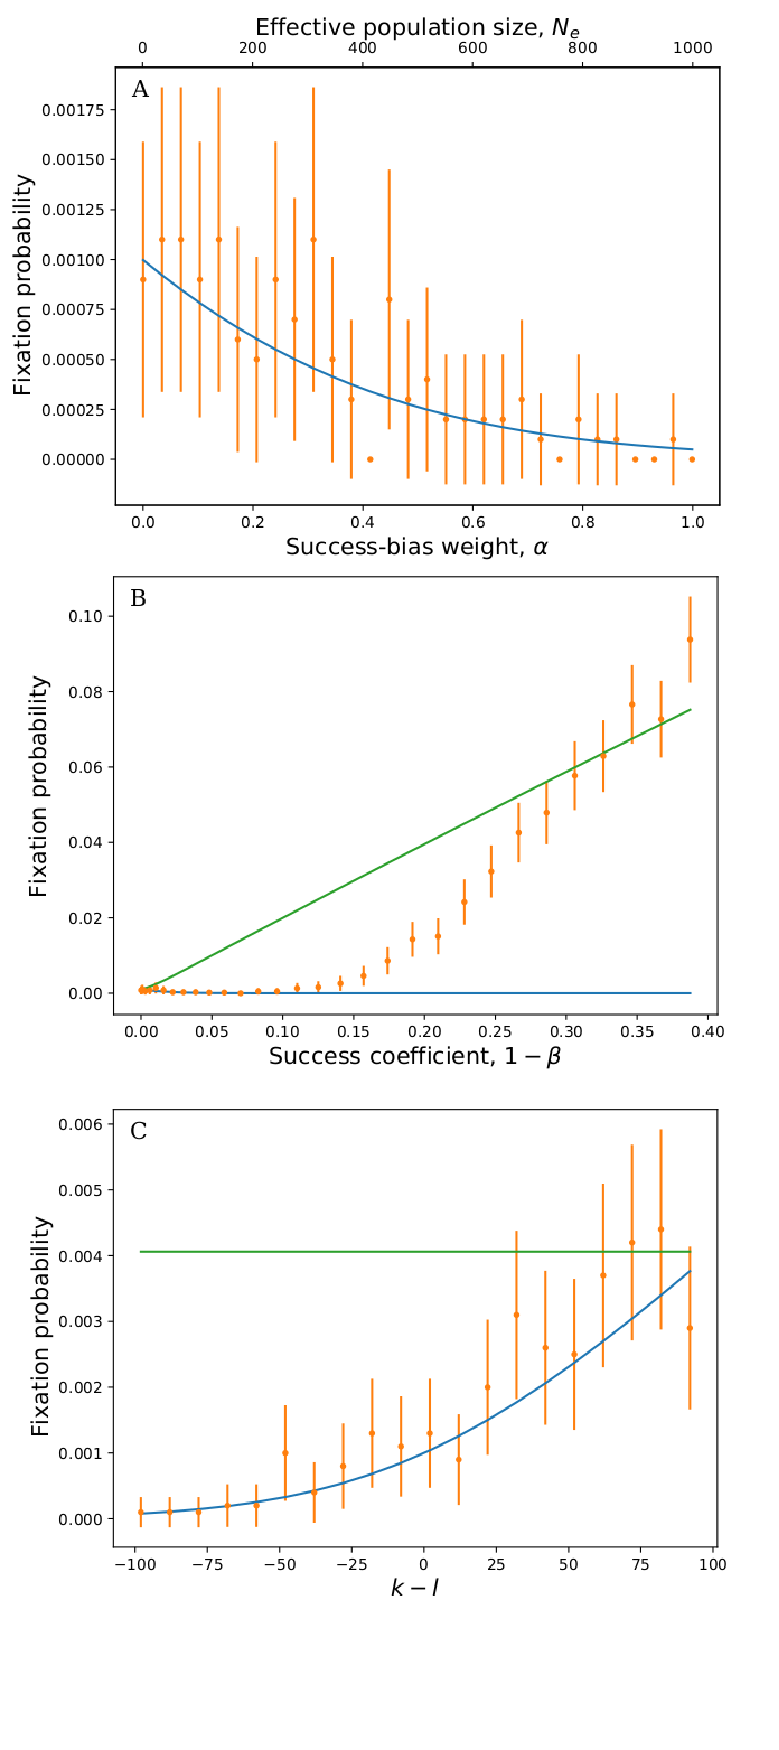
\includegraphics[width=\linewidth]{ch_env.pdf}
  \caption{\textbf{Fixation probability in a changing environment.}
\textbf{(A)} Fixation probability decreases with {the} success-bias weight (bottom x-axis) and effective population size (top x-axis). The approximation (blue; \cref{eq:ch_env}) agrees with simulation results (orange). 
\textbf{(B)} Fixation probability increases with the success coefficient, $\beta$.
When success bias is large ($1-\beta > 0.1$),  
simulation results (orange) are underestimated by the changing environment approximation (blue; \cref{eq:ch_env}). With even larger success bias ($1-\beta > 0.35$), even the constant environment approximation (green; \cref{eq:kimura_p}) slightly underestimates simulation results, likely because the diffusion equation approximation assumes weak "selection" .
(\textbf{C,D}) The approximation (blue) is robust to changes in environmental cycle length, as it agrees with simulations (orange) for different sizes of the changing environment cycle, where $k$ and $l$ are the number of generations each trait value is under success bias. 
When $k>l$, the approximation and the simulations are both very close to the constant environment approximation (green), because the more generations the rare phenotype is favored, the more similar it is to the constant environment model, where it is always favored by the success bias.
Markers show average of $10,000$ simulations, error bars show 75\% (panels A, C, and D) and 95\% (panel B) confidence intervals.
  Here, population size, $N=1,000$; phenotype values, $\hat{A}=1$ with $A=0.9$ (panels A and B) and $A=0.8$ (panels C and D); In panel A, the success coefficient is $1-\beta=s=0.005$; In panels B, C, and D, the success-bias weight is $\alpha=0.1$.
  }
  \label{fig:ch_env_alpha_beta}
\end{figure}


%%%%%%%%%%%%%%%%%%%%%%%%%%%%%%%%%%%%%%%%%%%%%%%%%%%%%%
% TODO MWF thinks the paper is better without this paragraph; if we remove, we should also remove references to it from abstac/intro/discussion
\subsection*{Adaptive success-bias weight}

We ran simulations of the role-model choice process during a single generation in which every copier evaluates its own optimal success-bias weight, $\alpha^*$, which minimizes the expected squared error between the estimated and the ideal trait values,
\begin{equation}
\alpha^* = \emph{argmin} \sum_{j=1}^N\frac{\alpha A_j + (1-\alpha) K_j}{\sum_{l=1}^N\alpha A_l + (1-\alpha) K_l} (\hat{A}-A_j)^2 \;,
\end{equation}
where $A_j$ is the trait of role-model $j$ and $K_j$ the number of copiers that already chose role-model $j$.

We find that when copiers {choose} their success-bias weight, it decreases with the number of copiers that have already chosen a role-model~(\Cref{fig:influence_advantage}).
Moreover, their estimation error is much lower compared to a constant success-bias weight, which gives roughly the same high estimation error to all copiers (compare \Cref{fig:influence_advantage}B and C): in this example, the adaptive weight estimation error converges to $0.046$, whereas a constant weight gives values $>0.74$.


\begin{figure}[h]
    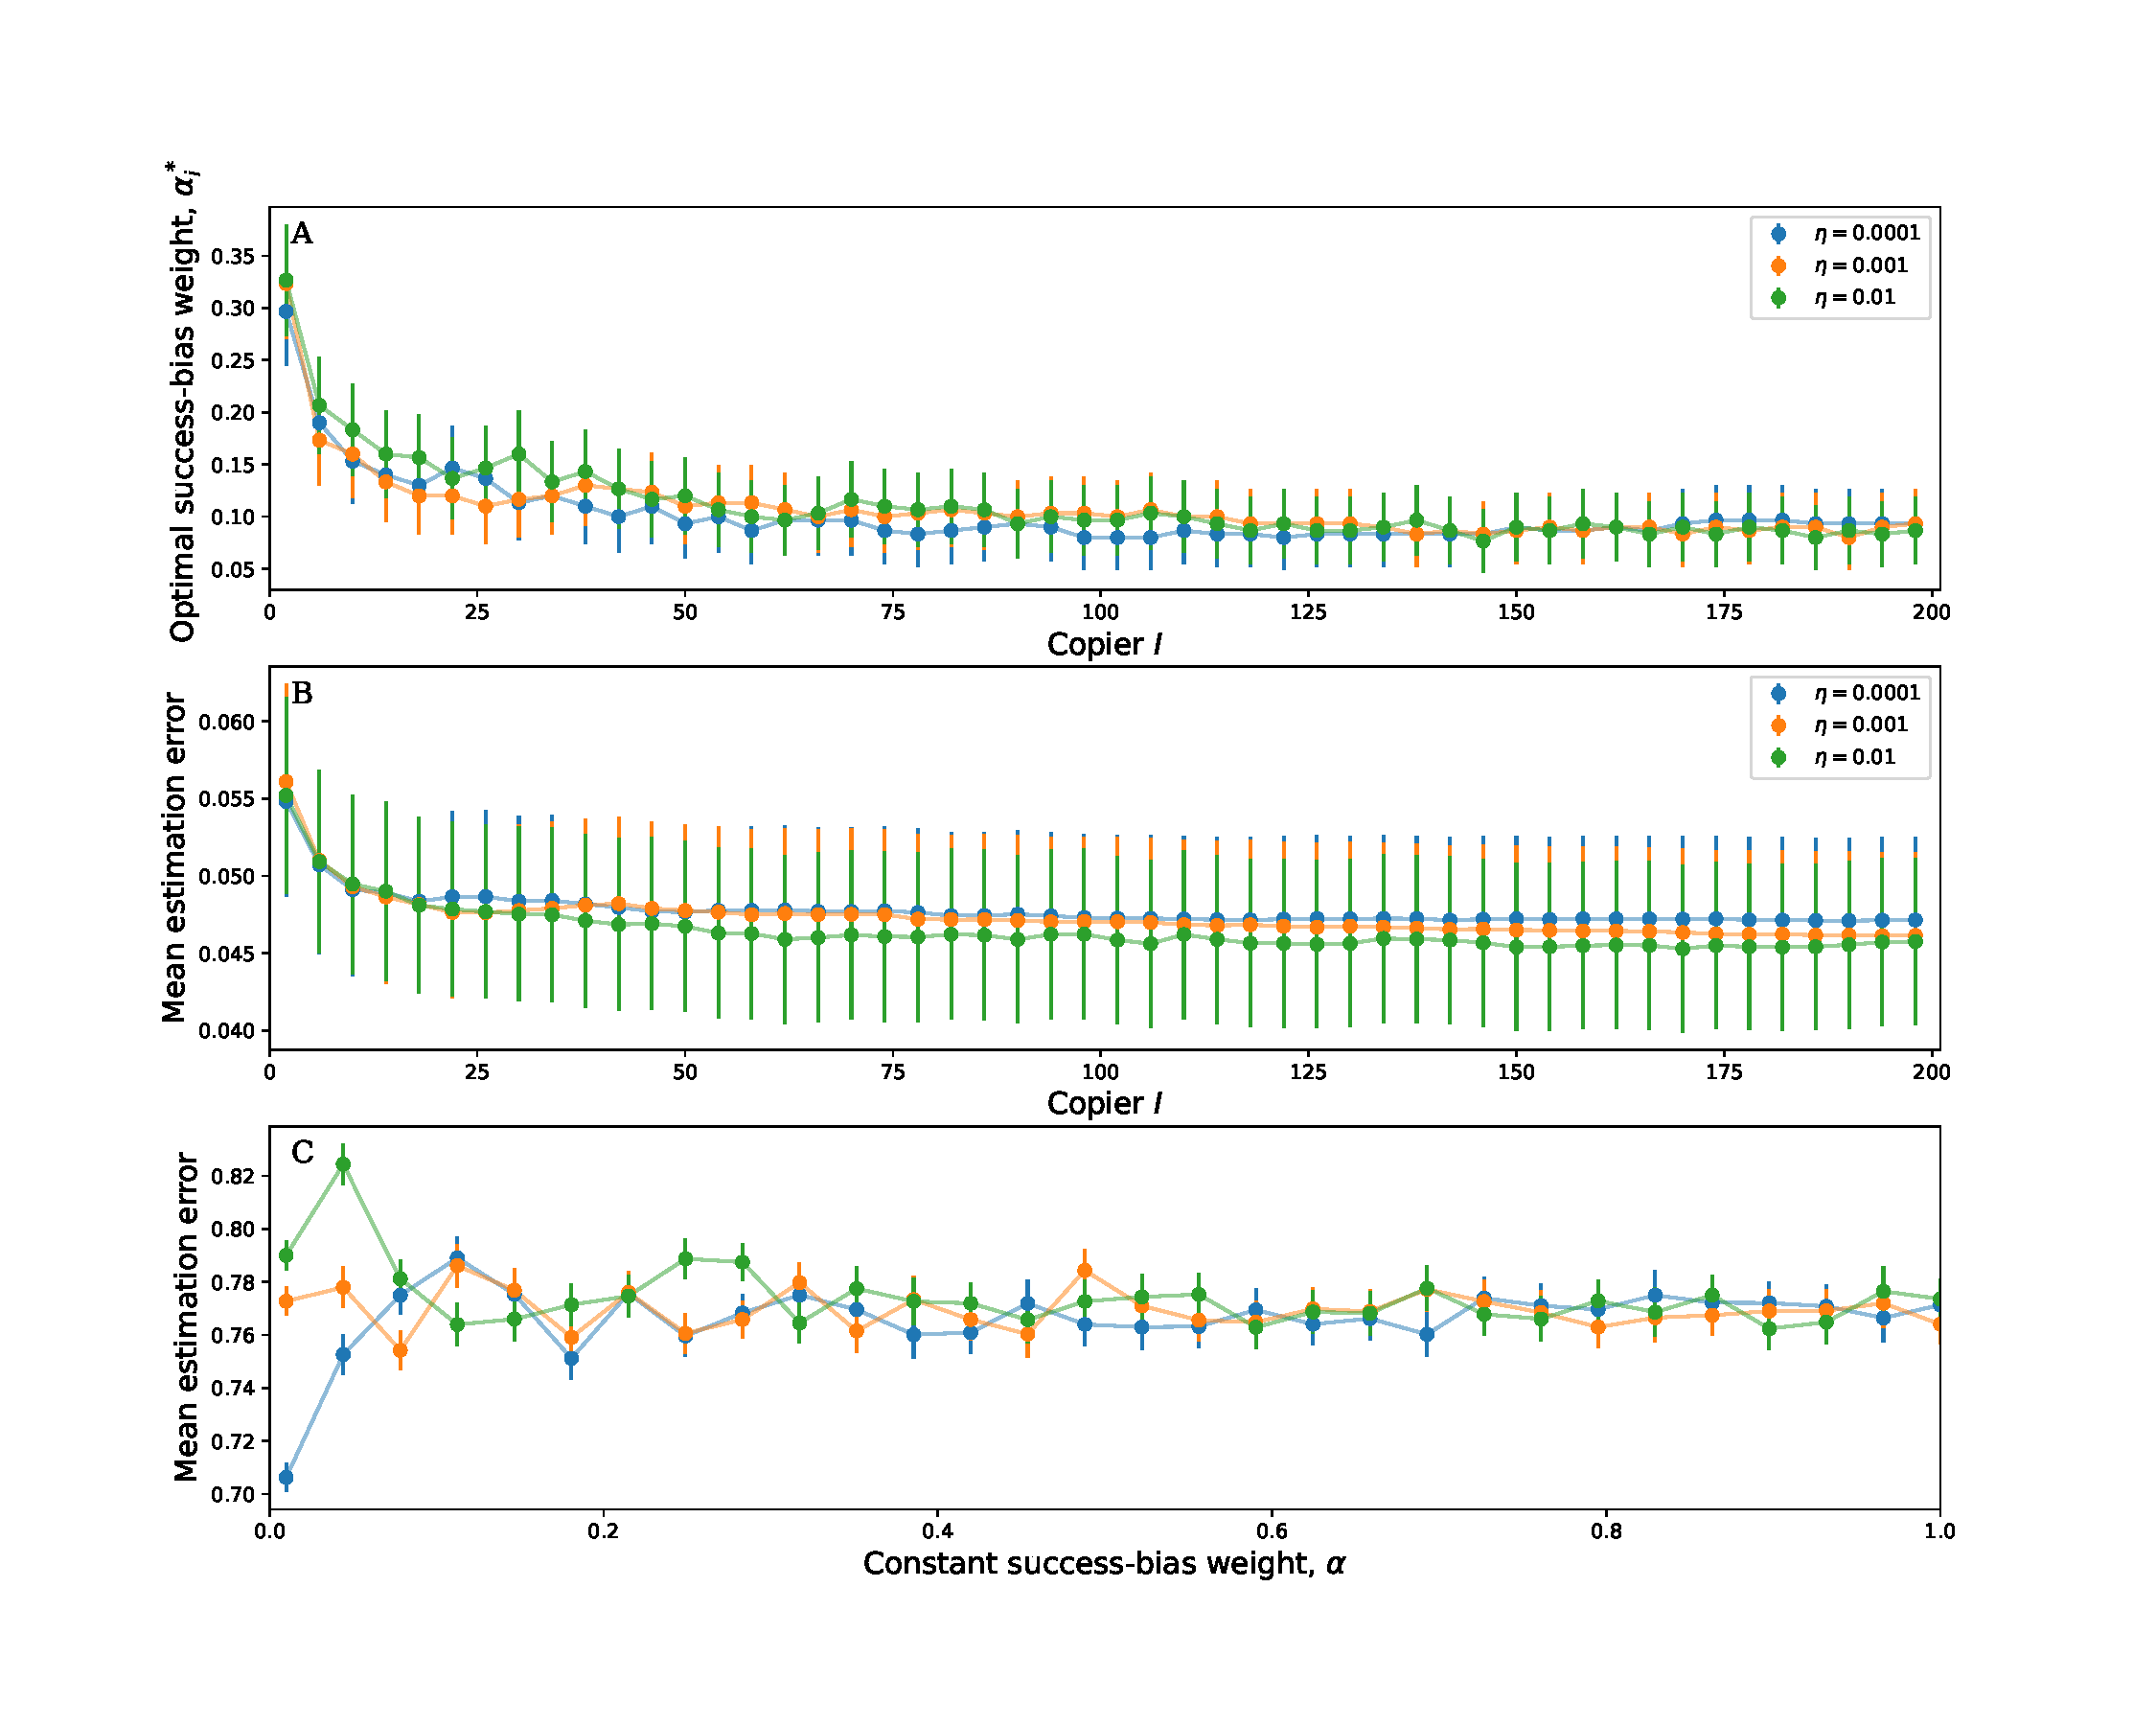
\includegraphics[width=\linewidth]{choose_bias.pdf}
  \caption{
  \textbf{Advantage of an adaptive success-bias weight.}
  Both success-bias weight $\alpha$ (\textbf{A}) and estimation error (\textbf{B}) decrease during the role-model choosing process, demonstrating that influence becomes more favored as more copiers have made their choice.
However, when $\alpha$ is homogeneous (\textbf{C}), the mean estimation error doesn't decrease, regardless of $\alpha$ or $\eta$.
The mean estimation error in the homogeneous $\alpha$ model is larger by a factor of $10$ than the adaptive $\alpha$ model.
Here, population size $N=200$; estimation error is normally distributed $e \sim N(0,\eta^2)$ with standard deviation $\eta=$0.0001 (blue), 0.001 (orange), 0.01 (green), plots are average of $300$ simulations.}	
  \label{fig:influence_advantage}
\end{figure}



%%%%%%%%%%%%%%%%%%%%%%%%%%%%%%%%%%%%%%%%%%%%%%%%%%%%%%
\section*{Discussion}
%During cultural transmission, cultural traits such as attitudes, values, beliefs, and behavioral patterns are transmitted between individuals, for example via copying and social learning.
{Some} cultural traits or cultural role-models may be copied more often {than others} due to transmission biases. 
{One such} bias is success bias, in which copiers are more likely to copy a successful role-model. {Although many} models assume that success can be accurately estimated{, it} has been suggested that because it is hard to estimate success, a more common bias is \emph{prestige bias}---a bias towards role-models perceived to be successful.
This perceived success can be determined by performance with respect to another trait (indirect) \citep{evolutionBook,fijian_social_bias}, or by the influence an individual has on others \citep{prestige_cultural_learning,prestige_evolution}.

We developed a cultural-evolution model with prestige bias that includes both indirect success and influence biases, where the latter is a bias towards role-models with many copiers {and hence is the same as conformity bias}.
We model the these biases using a stochastic role-model choice process: each copier, in {turn}, randomly chooses a role-model, and this choice is affected both by the estimated success of each potential role-model and the number of copiers that already chose each role-model (eq.~\ref{eq:prestige}). 

Hence, {our model has} two ``nested'' stochastic processes: the role-model choice process within each generation, and the cultural-evolutionary process between generations.
To simplify the mathematical and computational analysis, we developed analytic approximations for the role-model choice process using the the {\em generalized binomial distribution} (GBD, \Cref{res:GBD}) and the {\em Dirichlet-Multinomial distribution} (DM, \Cref{cor:dirichlet}).
The latter is especially useful, as it approximates the entire role-model choice process and only requires us to assume that the relative effect of success and influence is a characteristic of the role-model and not the copier.

Analyzing the model with the DM distribution, we found approximations for the fixation probability and fixation time of a cultural trait under biased transmission in a constant environment.
Our approximations are similar to Kimura's evolutionary-genetic approximations, {in} that (i) the difference between the resident and invading cultural trait values, $1-\beta(A)$, is equivalent to the selection coefficient in favor of a beneficial allele, $s$, and (ii) increasing the relative weight of influence versus success bias, $\alpha$, decreases the effective population size, $N_e$~(\Cref{fig:var_alpha}).

We also analyzed a cyclic changing environment in which the identity of the success-biased trait switches after a fixed amount of generations~(\Cref{fig:ch_env_alpha_beta}).
We find that, similarly to the constant environment approximation, a change in the success-bias weight $\alpha$ has no negative effects on the goodness-of-fit of the approximation to simulation results.
We also showed that this approximation is more sensitive to changes in the success coefficient $\beta$ than the constant environment approximation, and a lower value is required to have a good fit. The ratio between the number of {generations} in which the rare phenotype is under positive transmission bias and the number of generations in which it is under negative bias does not affect the goodness-of-fit of the approximation. 

We also examined a scenario in which copiers can adapt their success-weight bias, $\alpha$, to minimize their copying error, i.e., copy trait values closer to the optimal value.
We found that as the role-model choice process proceeds (that is, more copiers make their choices), both the success-bias weight ({chosen} by copiers) and the estimation error decrease. 
The latter is significantly lower {than in} a population using a constant, fixed success-bias weight, regardless of the value of the constant weight (\Cref{fig:influence_advantage}).
This suggests that the later a copier makes its choice, the more it should rely on choices of previous copiers, and the less it should rely on its own estimation.
The rationale, then, is that the more information a copier has, e.g., by using others as information sources, the more informative and effective his choice can be.

%\paragraph{Empirical evidence of prestige bias}
{Chudek et al.}\ \citep{prestige_cultural_learning} report the first direct tests in children that suggest the existence of prestige bias, defined as the tendency to learn from individuals to whom others have preferentially attended, learned, or deferred.
Their definition of prestige is similar to our influence bias. They showed that the odds of 3-4 years-old children learning from an adult role-model to whom bystanders had previously preferentially attended for 10 seconds were more than twice those of {learning from a role model} whom bystanders ignored.
They also note that prestige effects are domain sensitive: they found that prestigious role-models were attended more when demonstrating artifact use, whereas role-models presenting food preferences had less attendants, suggesting that the domain itself (artifact use vs. food preference) can affect the attendance, and hence the prestige of the role-model.
This {led to the suggestion} that when the trait is costly to learn individually, prestige will have a stronger bias \citep{prestige_cultural_learning}.
It would be interesting to include costs in our model to try and observe these effects and dynamics in a large population.

According to \citep{fijian_social_bias}, {natural} selection has favored the emergence of psychological biases for learning from those individuals most likely to possess adaptive information. 
{They} studied Fijian villages to examine if and how such biases emerge in a small-scale society.
They found that Fijian villagers are more likely to learn from role-models perceived as more successful/knowledgeable, both within and across domains.
Their research thus suggests that copying from those perceived as successful, rather than {who are actually} successful, is a common {phenomenon}. 
They show that the social networks representing copier--role-model relationships are centralized, suggesting that it is consistent with the prediction that people substantially share notions about who is a good cultural model, but that individuals' role-model selections are influenced by multiple factors.

{Prestige bias also occurs} in more modern domains such as western medicine.
Norredam and Album~\citep{medical_prestige} examined literature from 1950 to 2005 on the effects of prestige on medicinal practices. They found that active, specialized, biomedical, and high-technological types of medicine on organs in the upper part of the bodies of young and middle-aged people were accorded high levels of prestige, whereas medicine and practices that were not of these types had low levels of prestige.
For example, they found that surgery counts as the most prestigious specialty, while psychiatry is the {least} prestigious.
In addition, doctors tend to rank practices that require more time to master as more prestigious, while other procedures that are considered easier to master are less prestigious. 
This means that there may be very important practices that are neglected due to prestige bias.
They concluded that such differences in prestige may {affect} for actual priority setting in healthcare systems.

Prestige bias can help to cheaply estimate and acquire knowledge, which may facilitate survival and reproduction. However, it is not always the case, and there could be negative repercussions to this bias, such as invasion of maladaptive traits.
{Takahashi and Ihara} \citep{best_of_k} mention that social learning not only takes the form of random copying of other individuals, but also involves learners' choice of what to learn and from whom to learn. They suggest a best-of-k model where an individual samples~$k$ role-models and chooses the one he deems most "successful". They {mention} that a previous mathematical analysis has shown that it may sometimes result in maladaptive cultural evolution when the payoffs associated with cultural variants vary stochastically. In such a case, learners may be selectively disfavored and in the long run replaced by unbiased learners, who simply copy someone chosen at random. They developed new mathematical models that are simpler and mathematically tractable. They found that best-of-k learning, unlike unbiased learning, can facilitate the invasion of an on average inferior variant that sometimes gives a very high payoff {(see Fogarty et al.\ \citep{Fogarty2017} and references there)}. Our model, which includes influence bias, is consistent with this claim. When a maladaptive trait is ``piggybacking'' {on} a role-model with high influence, {the former} could spread in the population.
In addition, {best}-of-k learning can be stable against invasion by unbiased learning if social learning is sometimes combined with individual learning \citep{best_of_k}. 
Our model {includes only} social learning, and not individual learning, but it could be interesting to combine it with individual learning and see how it affects the dynamics.

Prestige bias can also accelerate reversal of harmful traditions such as child marriage and domestic violence. 
{Efferson et al.}\ \citep{harmful_traditions} suggest a \emph{spillover}  mechanism, in which an intervention affects a large enough group in a target population, so that others not included in the intervention also change their behavior.
They {find} that there are individuals who act as \emph{agents}, who are often {observed}, and therefore they are ideal targets for interventions. This is similar to influential role-models in our model, where a prestigious individual will be copied more often, and will therefore spread {their} trait faster and wider in the population.
They also suggest a way to use this {phenomenon} to change existing traditions in a population. It is very clear however, that just as it can be used to end harmful traditions, the same agents could start harmful traditions.


{Dunbar} \citep{social_brains} hypothesized that larger, more complex brains can store and manage more information and in turn, this information can support the costs of a larger brain.
Following {this, Muthukrishnan and Henrich \citep{collective_brains} suggested} that prestige can directly affect human physical evolution. They present a concept called \emph{cultural brains}---brains that evolved primarily for the acquisition of adaptive knowledge.
They then develop a model that predicts a strong relationship between brain size and group size, because group size also provides access to more adaptive knowledge. 
They also presented the \emph{cumulative cultural brain} hypothesis, which proposes that human brains have evolved with an ability and tendency for selective, high-fidelity social learning. As part of this process, there are a variety of strategies and biases that have evolved to hone in on the most adaptive knowledge. These strategies and biases include direct and indirect cues of the popularity of cultural traits (e.g. success and prestige biases).
They suggest that one of the reasons for the extreme increase in brain size in humans is the ability to "cheaply" acquire adaptive knowledge via transmission biases such as prestige.

%\paragraph{Further work.}
One path forward is an analysis of the dynamics of the adaptive success-bias weight model, in which every copier chooses its $\alpha$. It would be interesting to see the if the mean estimation error and the adaptive weight, $\alpha^*$, {converge} to specific values, and how they are affected by the model parameters.
It may also be possible to relax the assumptions required for our approximations, such as homogeneous estimation error and success-bias weight.
Lastly, it would be interesting to analyze the continuous model and determine how much it differs from the dichotomous model. 

Another way to expand our model is to account for the two types of prestige or leadership suggested by {Van Vugt and Smith} \citep{dual_leadership} that are attributed to Confucius and Machiavelli. Confucius viewed leaders as role-models who exercise influence through possessing superior knowledge, skills, and (outstanding) personal qualities. This fits the success bias in our model. 
In contrast, Machiavelli viewed leaders as rulers who exercise influence by imposing costs through (the threat of) punishment and violence. 
{Van Vugt and Smith suggest} that these opposing views are both partially supported by the available evidence but each one on its own offers an incomplete view of the complex and dynamic concept of leadership. 
Several adjustments could be made so that our model reflects these leadership styles, such as assuming there is a correlation between phenotype {and} leadership style. 
The {resulting} cultural-evolutionary dynamics and their dependence on the costs and benefits are intriguing.

\paragraph{Conclusions.}
{We} studied a model of cultural evolution under two transmission biases: the commonly studied success bias, together with influence bias, which has so far received less attention. We found approximations for this complex dynamics. We then showed that success bias affects the evolutionary dynamics much like natural selection does, whereas influence bias has a similar effect to random genetic drift. We also find a clear advantage to individuals that can choose the relative weight of the two biases.

{\small
\section*{Acknowledgements}
We thank Marc Feldman, Martin Pontz, Gili Greenbaum, Alon Rozen, and Tal Simon for discussions and comments.
This work was supported in part by 
Minerva Stiftung Center for Lab Evolution (YR) and  the John Templeton Foundation (YR 61809).
}

\section*{References}
\nolinenumbers
\begin{thebibliography}{}


\bibitem{fliesPaper}
  Battesti, Marine, et al. "Spread of social information and dynamics of social transmission within Drosophila groups." Current biology 22.4 (2012): 309-313.

\bibitem{transmissionVectors}
Creanza, Nicole, Oren Kolodny, and Marcus W. Feldman. "Cultural evolutionary theory: How culture evolves and why it matters." Proceedings of the National Academy of Sciences 114.30 (2017): 7782-7789.

\bibitem{negativeFrequency}
Aljadeff, Naama, Luc-Alain Giraldeau, and Arnon Lotem. "Competitive advantage of rare behaviours induces adaptive diversity rather than social conformity in skill learning." Proceedings of the Royal Society B 287.1933 (2020): 20201259.

\bibitem{transmissionVectorsBook}
Cavalli-Sforza, Luigi Luca, and Marcus W. Feldman. Cultural transmission and evolution: A quantitative approach. No. 16. Princeton University Press, 1981.

\bibitem{evolutionBook}
Boyd, Robert, and Peter J. Richerson. Culture and the evolutionary process. University of Chicago press, 1988.

\bibitem{complexityPaper}
Fogarty, Laurel, et al. "The driving forces of cultural complexity: neanderthals, modern humans, and the question of population size." Human Nature 28 (2017): 39-52.

\bibitem{strategiesPaper}
Rendell, Luke, et al. "Why copy others? Insights from the social learning strategies tournament." Science 328.5975 (2010): 208-213.

\bibitem{sexualSelectionBook}
Andersson, Malte, and Yoh Iwasa. "Sexual selection." Trends in ecology \& evolution 11.2 (1996): 53-58.

\bibitem{chimpsCopy}
Kendal, Rachel, et al. "Chimpanzees copy dominant and knowledgeable individuals: implications for cultural diversity." Evolution and Human Behavior 36.1 (2015): 65-72.

\bibitem{chimpsPrestige}
Horner, Victoria, et al. "Prestige affects cultural learning in chimpanzees." PloS one 5.5 (2010): e10625.

\bibitem{dualEvolution}
Henrich, Joseph, and Richard McElreath. "Dual-inheritance theory: the evolution of human cultural capacities and cultural evolution." (2007).

\bibitem{elepahntsRepo}
McComb, Karen, et al. "Matriarchs as repositories of social knowledge in African elephants." Science 292.5516 (2001): 491-494.

\bibitem{wtfGene}
Eickbush, Michael T., Janet M. Young, and Sarah E. Zanders. "Killer meiotic drive and dynamic evolution of the wtf gene family." Molecular Biology and Evolution 36.6 (2019): 1201-1214.

\bibitem{pageRank}
Xing, Wenpu, and Ali Ghorbani. "Weighted pagerank algorithm." Proceedings. Second Annual Conference on Communication Networks and Services Research, 2004.. IEEE, 2004.

\bibitem{conformism}
Molleman, Lucas, Ido Pen, and Franz J. Weissing. "Effects of conformism on the cultural evolution of social behaviour." PloS one 8.7 (2013): e68153.

\bibitem{GBD}
Drezner, Zvi, and Nicholas Farnum. "A generalized binomial distribution." Communications in Statistics-Theory and Methods 22.11 (1993): 3051-3063.

\bibitem{dirichlet}
Frigyik, Bela A., Amol Kapila, and Maya R. Gupta. "Introduction to the Dirichlet distribution and related processes." Department of Electrical Engineering, University of Washignton, UWEETR-2010-0006 6 (2010): 1-27.

\bibitem{martingaleBook}
Durrett, Richard, and R. Durrett. Essentials of stochastic processes. Vol. 1. New York: Springer, 1999.

\bibitem{kimura}
Kimura, Motoo. "On the probability of fixation of mutant genes in a population." Genetics 47.6 (1962): 713.

\bibitem{durret}
Durrett, Richard, and Richard Durrett. Probability models for DNA sequence evolution. Vol. 2. New York: Springer, 2008.

\bibitem{changeEnv}
Ram, Yoav, Uri Liberman, and Marcus W. Feldman. "Evolution of vertical and oblique transmission under fluctuating selection." Proceedings of the National Academy of Sciences 115.6 (2018): E1174-E1183.

\bibitem{animal_leadership}
King, Andrew J., and Guy Cowlishaw. "Leaders, followers, and group decision-making." Communicative \& integrative biology 2.2 (2009): 147-150.

\bibitem{dual_leadership}
Van Vugt, Mark, and Jennifer E. Smith. "A dual model of leadership and hierarchy: Evolutionary synthesis." Trends in Cognitive Sciences 23.11 (2019): 952-967.

\bibitem{fijian_social_bias}
Henrich, Joseph, and James Broesch. "On the nature of cultural transmission networks: evidence from Fijian villages for adaptive learning biases." Philosophical Transactions of the Royal Society B: Biological Sciences 366.1567 (2011): 1139-1148.

\bibitem{harmful_traditions}
Efferson, Charles, Sonja Vogt, and Ernst Fehr. "The promise and the peril of using social influence to reverse harmful traditions." Nature human behaviour 4.1 (2020): 55-68.

\bibitem{prestige_evolution}
Henrich, Joseph, and Francisco J. Gil-White. "The evolution of prestige: Freely conferred deference as a mechanism for enhancing the benefits of cultural transmission." Evolution and human behavior 22.3 (2001): 165-196.

\bibitem{best_of_k}
Takahashi, Takuya, and Yasuo Ihara. "Cultural and evolutionary dynamics with best-of-k learning when payoffs are uncertain." Theoretical Population Biology 128 (2019): 27-38.

\bibitem{medical_prestige}
Norredam, Marie, and Dag Album. "Prestige and its significance for medical specialties and diseases." Scandinavian journal of public health 35.6 (2007): 655-661.

\bibitem{collective_brains}
Muthukrishna, Michael, and Joseph Henrich. "Innovation in the collective brain." Philosophical Transactions of the Royal Society B: Biological Sciences 371.1690 (2016): 20150192.

\bibitem{social_brains}
Dunbar, Robin IM. "The social brain hypothesis and its implications for social evolution." Annals of human biology 36.5 (2009): 562-572.

\bibitem{prestige_cultural_learning}
Chudek, Maciej, et al. "Prestige-biased cultural learning: Bystander's differential attention to potential models influences children's learning." Evolution and human behavior 33.1 (2012): 46-56.

\bibitem{evolution_of_cultural_evolution}
Henrich, Joseph, and Richard McElreath. "The evolution of cultural evolution." Evolutionary Anthropology: Issues, News, and Reviews: Issues, News, and Reviews 12.3 (2003): 123-135.

\bibitem{cultural_traits}
O'Brien, Michael J., et al. "Cultural traits as units of analysis." Philosophical Transactions of the Royal Society B: Biological Sciences 365.1559 (2010): 3797-3806.

\bibitem{dolphins_whales}
Whitehead, Hal. "Gene–culture coevolution in whales and dolphins." Proceedings of the National Academy of Sciences 114.30 (2017): 7814-7821.

\bibitem{cooperation}
Cohen, Dor, et al. "Non-vertical cultural transmission, assortment and the evolution of cooperation." Proceedings of the Royal Society B 288.1951 (2021): 20203162.

\bibitem{conformity}
Denton, Kaleda K., Yoav Ram, and Marcus W. Feldman. "Conformity and content-biased cultural transmission in the evolution of altruism." Theoretical Population Biology 143 (2022): 52-61.

\bibitem{anticonformity}
Denton, Kaleda Krebs, et al. "Cultural evolution of conformity and anticonformity." Proceedings of the National Academy of Sciences 117.24 (2020): 13603-13614.

\bibitem{facebook_marketing}
Lee, Woojin, Lina Xiong, and Clark Hu. "The effect of Facebook users’ arousal and valence on intention to go to the festival: Applying an extension of the technology acceptance model." International Journal of Hospitality Management 31.3 (2012): 819-827.

\bibitem{social_influence}
Anagnostopoulos, Aris, Ravi Kumar, and Mohammad Mahdian. "Influence and correlation in social networks." Proceedings of the 14th ACM SIGKDD international conference on Knowledge discovery and data mining. 2008.

\bibitem{influence_analysis}
Peng, Sancheng, et al. "Influence analysis in social networks: A survey." Journal of Network and Computer Applications 106 (2018): 17-32.

\bibitem{social_media}
Diga, Marichris, and Tom Kelleher. "Social media use, perceptions of decision-making power, and public relations roles." Public Relations Review 35.4 (2009): 440-442.

\bibitem{python}
Van Rossum, Guido. "Python Programming Language." USENIX annual technical conference. Vol. 41. No. 1. 2007.

\bibitem{numpy}
Van Der Walt, Stefan, S. Chris Colbert, and Gael Varoquaux. "The NumPy array: a structure for efficient numerical computation." Computing in science \& engineering 13.2 (2011): 22-30.

\bibitem{mathplotlib}
Hunter, John D. "Matplotlib: A 2D graphics environment." Computing in science \& engineering 9.03 (2007): 90-95.

\bibitem{kimura_average}
Kimura, Motoo, and Tomoko Ohta. "The average number of generations until fixation of a mutant gene in a finite population." Genetics 61.3 (1969): 763.

\bibitem{otto_fixation}
Slatkin, Montgomery. "Fixation probabilities and fixation times in a subdivided population." Evolution (1981): 477-488.

\bibitem{lemurs}
Erhart, Elizabeth M., and Deborah J. Overdorff. "Female coordination of group travel in wild Propithecus and Eulemur." International Journal of Primatology 20 (1999): 927-940.

\bibitem{no_replication}
Boyd, Robert, and Joseph Henrich. "On modeling cognition and culture: Why cultural evolution does not require replication of representations." Journal of cognition and culture 2.2 (2002): 87-112.

\bibitem{kin_selection}
Gardner, Andy, Stuart A. West, and Geoff Wild. "The genetical theory of kin selection." Journal of evolutionary biology 24.5 (2011): 1020-1043.

\bibitem{Truskanov2020}
Truskanov, Noa, Yasmin Emery, and Redouan Bshary. "Juvenile cleaner fish can socially learn the consequences of cheating." Nature communications 11.1 (2020): 1159.

\bibitem{Kolodny2022}
Kolodny, Oren, et al. "Differential application of cultural practices at the family and individual levels may alter heritability estimates." Behavioral and Brain Sciences 45 (2022): e167.

\bibitem{Denton2021}
Denton, Kaleda K., Uri Liberman, and Marcus W. Feldman. "On randomly changing conformity bias in cultural transmission." Proceedings of the National Academy of Sciences 118.34 (2021): e2107204118.

\bibitem{Borofsky2022}
Borofsky, Talia, and Marcus W. Feldman. "Success-biased social learning in a one-consumer, two-resource model." Theoretical Population Biology 146 (2022): 29-35.

\bibitem{Mesoudi2008}
The cultural transmission of great basin projectile-point technology II: An agent-based computer simulation

\bibitem{Lehmann2009}
Lehmann, L., and M.W. Feldman. Coevolution of adaptive technology, maladaptive culture, and population size in a producer-scrounger game. Proc.\ Roy.\ Soc.\ B 276 (2009): 3853-3862.

\bibitem{Fogarty2017}Fogarty, L., J. Y. Wakano, M. W. Feldman, and K. Aoki. The driving forces of cultural complexity: Neanderthals, modern humans, and the question of population size. Hum.\ Nat.\ (2017): 28: 39-52.

\bibitem{cumul_culture}Denton, Kaleda K, Yoav Ram, and Marcus W. Feldman. 2023. “Conditions That Favour Cumulative Cultural Evolution.” Philosophical Transactions of the Royal Society B: Biological Sciences 378 (1872). https://doi.org/10.1098/rstb.2021.0400.


\end{thebibliography}

\pagebreak

\begin{appendices}
\renewcommand{\theequation}{\thesection\arabic{equation}}
\counterwithin*{equation}{section}

%%%%%%%%%%%%%%%%%%%%%%%%%%%%%%%%%%
\section{General binomial distribution approximation} \label{sec:GBD}

\paragraph{Proving $\E[K_{Nj}] = \alpha_j \cdot \beta(A_j+e) / \overline{\alpha \cdot \beta(A+e)}$, where the {average} in the denominator is over the role-models index, $j$.}


\begin{proof}
The initial prestige of role-model $j$ based on \cref{eq:prestige} is
\begin{equation}\label{eq:initial_prob}
G_{1,j} = \frac{\alpha_j\cdot\beta(A_j+e)}{\sum\limits_{m=1}^{N} \alpha_m\cdot\beta(A_m+e)} \;.
\end{equation}
The denominator of \cref{eq:initial_prob} can also be formulated as:
\begin{equation}\label{eq:denominator}
 \sum\limits_{m=1}^{N}\alpha_m\beta(A_m+e) = N \cdot \overline{\alpha \cdot \beta(A+e)} \;,
\end{equation}
where $\overline{\alpha\beta(A+e)}$ is the mean value of $\alpha_m\cdot\beta(A_m+e)$.
Using \cref{eq:denominator} and \textbf{Corollary 1} we get,
\begin{equation}
\E[K_{N,j}] = \alpha_j \cdot \beta(A_j+e) \bigg/ \overline{\alpha \cdot \beta(A+e)} \;,
\end{equation}
\end{proof}

\section{Drift and diffusion in a constant environment} \label{sec:drift_diff_const}

\paragraph{Proving drift and diffusion terms in a constant environment.}
Let $x$ and $x'$ be the frequency of type $\hat{A}$ in a population with $N$ individuals in the current and next generation, and  $\beta$ {be} the success coefficient of phenotype $A$, $\beta = \beta(A) < \beta(\hat{A}) = 1$.
Then,
\begin{equation*}
E[x'-x] \approx x(1-x)(1-\beta) \;, 
\quad
V(x'-x) \approx x(1-x)\Big(\frac{1}{\alpha N + (1-\alpha)}\Big) \;.
\end{equation*} 


\begin{proof}
Let $X$ be the number of individuals of type $\hat{A}$ such that $x=X/N$. $X'$ is the number of individuals with $\hat{A}$ in the next generation.
The expected number of individuals is (due to the DM approximation),
\begin{equation}
E[X'] = N  \frac{\alpha_1}{\alpha_1+\alpha_2} \;,
\end{equation}
where $\alpha_1 = \alpha' X$ and $\alpha_2 = \alpha'(N-X)\beta$, from  \cref{eq:binary-model}.
To use frequencies instead of counts, $E[x'] = E[X'/N] = \frac{1}{N}E[X']$.
Putting it together,
\begin{equation}
\begin{split}
E[x'] &= \frac{1}{N}N\frac{\alpha' xN}{\alpha' xN + \alpha' N (1-x)\beta}
	  = \frac{x}{x + (1-x)\beta} \\
	  &= \frac{x}{x + (1-x) -(1-x) + (1-x)\beta}
	  = x \frac{1}{1 -(1-x)(1-\beta)}  \\
	  &= x \big(1 + (1-x)(1-\beta) + o(1-\beta)\big)
	  = x + x(1-x)(1-\beta) + o(1-\beta) \;, 
\end{split}
\end{equation}
following Durrett~\citep[p.~253, ch~7.2]{durret} and because $1/(1-y)=1+y+y^2+\ldots$.

%By definition, $x$ is constant, so $E[x] = x$.
{We} therefore have
\begin{equation}\label{eq:expec_freq}
E[x'-x] = E[x'] - E[x] = x(1-x)(1-\beta) + o(1-\beta) \;,
\end{equation}
which gives us the drift term of the diffusion equation.

Using the variance of the DM distribution,
\begin{equation}
V(X') = N\frac{\alpha_1}{\alpha_1+\alpha_2}
\Big(1-\frac{\alpha_1}{\alpha_1+\alpha_2}\Big)
\Big(\frac{N + \alpha_1+\alpha_2}{1+\alpha_1+\alpha_2}\Big) \;.
\end{equation}
Again, we want to use frequencies so we have $V(X'/N) = \frac{1}{N^2}V(x')$.
Putting it together with our model notations,
\begin{equation}
V(x') = \frac{1}{N^2}N\frac{x}{x+(1-x)\beta}\Big(1-\frac{x}{x+(1-x)\beta}\Big)
\Big(\frac{N + \alpha' xN + \alpha' N(1-x)\beta}{1 + \alpha' xN + \alpha' N(1-x)\beta}\Big) \;.
\end{equation}

Following Durrett~\citep[ch~7.2]{durret}, we assume $\beta \approx 1$, such that
\begin{equation}
\frac{x}{x + (1-x)\beta} \approx x \,
\end{equation}
and for the entire variance expression we get
\begin{equation}
%\begin{split}
V(x') \approx  \frac{1}{N} x(1-x)
\Big(\frac{N + \alpha' xN + \alpha' N - \alpha' xN}{1 + \alpha' xN + \alpha' N - \alpha' xN}\Big)
= x(1-x)\Big(\frac{1 + \alpha'}{1 + \alpha' N}\Big) \;.
%\end{split}
\end{equation}
The current frequency $x$ is a given, such that $V(x) = 0$,
and therefore
\begin{equation}\label{eq:var_diff_durret}
V(x'-x) = V(x') - V(x) \approx  x(1-x)(\frac{1 + \alpha'}{1 + \alpha' N}) \;.
\end{equation}
$\alpha'$ is the odds ratio of the bias weight, 
\begin{equation}\label{eq:success_ratio}
\alpha' = \frac{\alpha}{1-\alpha} \;.
\end{equation}
Combining \cref{eq:var_diff_durret} and \cref{eq:success_ratio} we get:
\begin{equation}\label{eq:const_var}
\begin{split}
V(x'-x) \approx x(1-x)\Big(\frac{1 + \frac{\alpha}{1-\alpha}}{1 + \frac{\alpha}{1-\alpha} N}\Big)
% &= x(1-x)(\frac{\frac{1-\alpha+\alpha}{1-\alpha}}{\frac{1-\alpha+\alpha N}{1-\alpha}})\\
% &= x(1-x)(\frac{1}{1- \alpha(1-N)})\\
  = x(1-x)(\frac{1}{\alpha N + (1-\alpha)}) \;.
\end{split}
\end{equation}
This gives the diffusion term of the diffusion equation.
\end{proof}

\section{Drift and diffusion in a changing environment} \label{sec:drift_diff_chang}
\paragraph{Proving drift and diffusion terms in a changing environment.}
Let $x$ be the initial frequency of the invading phenotype and $X_t$ is the number of individuals with the phenotype at time $t$.
Then,
\begin{equation*}
E[X_t/N - x] \simeq x(1-x) S_t / N_e \;, 
\quad
\text{and}
\quad
V(X_t/N-x) \simeq  t x(1-x) / N_e \;,
\end{equation*}
where $S_t=\sum\limits_{i=1}^{t} N (1-\beta_t)$.


\begin{proof}
Let $s_t=N(1-\beta_t)$, and $S_n=\sum\limits_{i=1}^n s_i$, where $\beta_t$ is $\beta(A)$ at generation $t$.
We prove by induction both terms in \cref{eq:ch_expected_and_var}.
From \cref{eq:expec_freq} we know that
\begin{equation}\label{eq:ch_1}
%\begin{split}
E\left[\frac{X_{t+1}}{N}-\frac{X_t}{N}\bigg|X_t\right] 
= \frac{X_t}{N}\left(1-\frac{X_t}{N}\right)(1-\beta_{t+1}) 
= \frac{1}{N}\frac{X_t}{N}\left(1-\frac{X_t}{N}\right)s_{t+1} \;.
%\end{split}
\end{equation}
Also note that using the definition of $V(y)=E[y^2]-(E[y])^2$
\begin{equation}
\begin{split}
E\left[\frac{X_t}{N}\left(1-\frac{X_t}{N}\right)\right] 
&= E\left[\frac{X_t}{N}-\left(\frac{X_t}{N}\right)^2\right] 
= E\left[\frac{X_t}{N}\right] - E\left[\left(\frac{X_t}{N}\right)^2\right] \\
&= E\left[\frac{X_t}{N}\right] - V\left(\frac{X_t}{N}\right) - \left(E\left[\frac{X_t}{N}\right]\right)^2 \;.
\end{split}
\end{equation}

We can now use the induction assumption of $V\big(\frac{X_t}{N}\big)$ to get
\begin{equation}
\begin{split}
E\left[\frac{X_t}{N}\left(1-\frac{X_t}{N}\right)\right] 
&\simeq E\left[\frac{X_t}{N}\right]\left(1-E\left[\frac{X_t}{N}\right]\right)-\frac{1}{N_e}tx(1-x) \;.
\end{split}
\end{equation}
From \cref{eq:ch_1} we know that
\begin{equation}
\begin{split}
E\left[\frac{X_{t+1}}{N}-\frac{X_t}{N}\right] 
&= \frac{1}{N}s_{t+1}E\left[\frac{X_t}{N}\left(1-\frac{X_t}{N}\right)\right] 
\simeq \frac{1}{N}s_{t+1}\left(E\left[\frac{X_t}{N}\right]\left(1-E\left[\frac{X_t}{N}\right]\right) - \frac{1}{N_e}tx(1-x)\right) \\
&\simeq \frac{1}{N}s_{t+1}\cdot E\left[\frac{X_t}{N}\right]\left(1-E\left[\frac{X_t}{N}\right]\right) - \frac{1}{N_e N}s_{t+1}tx(1-x) \;.
\end{split}
\end{equation}
Now we omit $O\big(\frac{1}{Ne\cdot N}\big)$ and get
\begin{equation}\label{eq:ch_2}
E\left[\frac{X_{t+1}}{N}-\frac{X_t}{N}\right] \simeq \frac{1}{N}s_{t+1}\cdot E\left[\frac{X_t}{N}\right]\left(1-E\left[\frac{X_t}{N}\right]\right) \;.
\end{equation}

We now look at the induction assumption to see that
\begin{equation}
E\left[\frac{X_t}{N}-x\right]
= E\left[\frac{X_t}{N}\right]-E[x]
= E\left[\frac{X_t}{N}\right]-x \;,
\end{equation}
so using the assumption we get
\begin{equation}
\begin{split}
E\left[\frac{X_t}{N}\right] 
&\simeq \frac{1}{N} S_t x(1-x)+x \;, \\
1 - E\left[\frac{X_t}{N}\right] 
&\simeq 1- \frac{1}{N} S_t x(1-x)+x \;.
\end{split}
\end{equation}
We use both expressions in \cref{eq:ch_2} and get
\begin{equation}\label{eq:ch_3}
\begin{split}
E\left[\frac{X_{t+1}}{N}-\frac{X_t}{N}\right] 
&\simeq \frac{1}{N}s_{t+1} \left(\frac{1}{N} S_t x(1-x)+x \right)\left(1- \frac{1}{N} S_t x(1-x)+x \right) \\
&\simeq  \frac{1}{N}s_{t+1}\cdot x(1-x) \;,
\end{split}
\end{equation}
after again omitting $O\big(\frac{1}{N^2}\big)$ terms.
To conclude the proof, we note that
\begin{equation}
E\left[\frac{X_{t+1}}{N}-x\right] 
= E\left[\frac{X_{t+1}}{N}-\frac{X_t}{N}\right] + E\left[\frac{X_t}{N}-x\right] \;,
\end{equation}
so again using the induction assumption, together with \cref{eq:ch_3} we get
\begin{equation}
\begin{split}
E\left[\frac{X_{t+1}}{N}-x\right] \simeq \frac{1}{N}s_{t+1}\cdot x(1-x) + \frac{1}{N}S_t\cdot x(1-x) \\
\simeq \frac{1}{N}x(1-x)(S_t + s_{t+1}) 
\simeq \frac{1}{N} S_{t+1} x(1-x) \;,
\end{split}
\end{equation}
which proves the drift term.

For the diffusion term, we use a property of variance,
\begin{equation}\label{eq:ch_var}
V\left(\frac{X_{t+1}}{N}\right) 
= E\left[V\left(\frac{X_{t+1}}{N} \bigg|X_t \right)\right] + V\left(E\left[\frac{X_{t+1}}{N} \bigg|X_t \right]\right) \;.
\end{equation}

Using \cref{eq:ch_1} we see that
\begin{equation}\label{eq:ch_var1}
\begin{split}
&E\left[\frac{X_{t+1}}{N} \bigg|X_t \right] - E\left[\frac{X_{t}}{N} \bigg|X_t \right] 
= \frac{1}{N}s_{t+1}\frac{X_t}{N}\left(1-\frac{X_t}{N} \right) \\
&E\left[\frac{X_{t+1}}{N} \bigg|X_t \right] 
= \frac{X_t}{N} + \frac{1}{N}s_{t+1}\frac{X_t}{N}\left(1-\frac{X_t}{N} \right) \;.
\end{split}
\end{equation}

Using \cref{eq:const_var} we get
\begin{equation}
V\left(\frac{X_{t+1}}{N} \bigg|X_t \right) 
= \frac{1}{N_e}\frac{X_t}{N}\left(1-\frac{X_t}{N} \right) \;,
\end{equation}
and using the equation $y'(1-y') \simeq y(1-y)$ on the first part of \cref{eq:ch_var} we get
\begin{equation}\label{eq:ch_var2}
E\left[V\left(\frac{X_{t+1}}{N} \bigg|X_t \right)\right] 
= \frac{1}{N_e}E\left[\frac{X_t}{N}\left(1- \frac{X_t}{N}\right) \right] \simeq \frac{1}{N_e} x(1-x) \;.
\end{equation}
Moving on to simplify the second part of \cref{eq:ch_var} using \cref{eq:ch_var1},
\begin{equation}
V\left(E\left[\frac{X_{t+1}}{N} \bigg|X_t \right]\right) 
= V\left(\frac{X_t}{N} + \frac{1}{N}s_{t+1}\frac{X_t}{N}\left(1-\frac{X_t}{N} \;.\right) \right)
\end{equation}
Now, because $\frac{X_t}{N}$ is a frequency, i.e $0 \leq X_t/N \leq 1$, we know that $V\left(\frac{X_t}{N}\left(1-\frac{X_t}{N} \right) \right)\leq\frac{1}{4}$. We therefore find that
\begin{equation}
V\left(\frac{1}{N}s_{t+1}\frac{X_t}{N}\left(1-\frac{X_t}{N} \right) \right)
\leq \frac{1}{4N^2}s^2_{t+1} ;,
\end{equation}
and so it can be ignored.
Combining our equations we get
\begin{equation}
V\left(E\left[\frac{X_{t+1}}{N} \bigg|X_t \right]\right) 
= V\left(\frac{X_t}{N}\right) + O\left(\frac{1}{N^2}\right)\simeq V\left(\frac{X_t}{N}\right) \;.
\end{equation}
Using the induction assumption and \cref{eq:ch_var2},
\begin{equation}
V\left(\frac{X_{t+1}}{N}\right) 
\simeq \frac{1}{N_e}x(1-x) + \frac{1}{N_e}tx(1-x) \simeq \frac{1}{N_e}x(1-x)(t+1) \,
\end{equation}
which proves the diffusion term.
\end{proof}
\end{appendices}

%%%

\newpage
\section*{Supplementary Figures}
\beginsupplement % https://support.authorea.com/en-us/article/how-to-create-an-appendix-section-or-supplementary-information-1g25i5a/

\begin{figure}[h]
    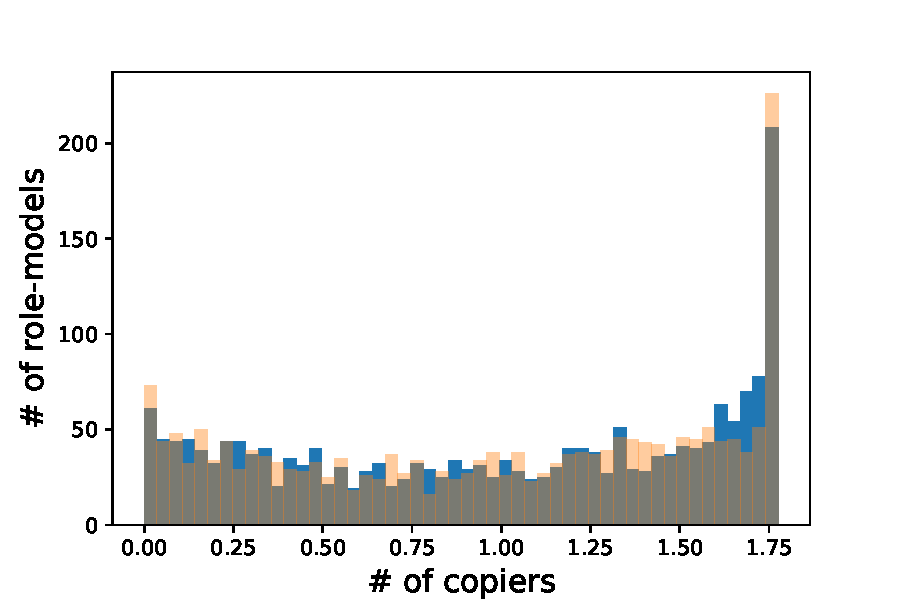
\includegraphics[width=0.7\linewidth]{GBD_validation.pdf}
  \caption{
  \textbf{Numerical validation of the GB approximation.}
  The approximation (orange) fits simulation results (blue) well when using 1,000 simulations. 
  Here, population size, $N=2,000$; bias weight, $\alpha=0.1$; {ideal} phenotype value, $\hat{A}=1$; role-model traits $\vec{A} \sim N(0,1)$; success bias value, $\beta(A)=0.956$.}	
  \label{fig:GBD}
\end{figure}


\begin{figure}[h]
    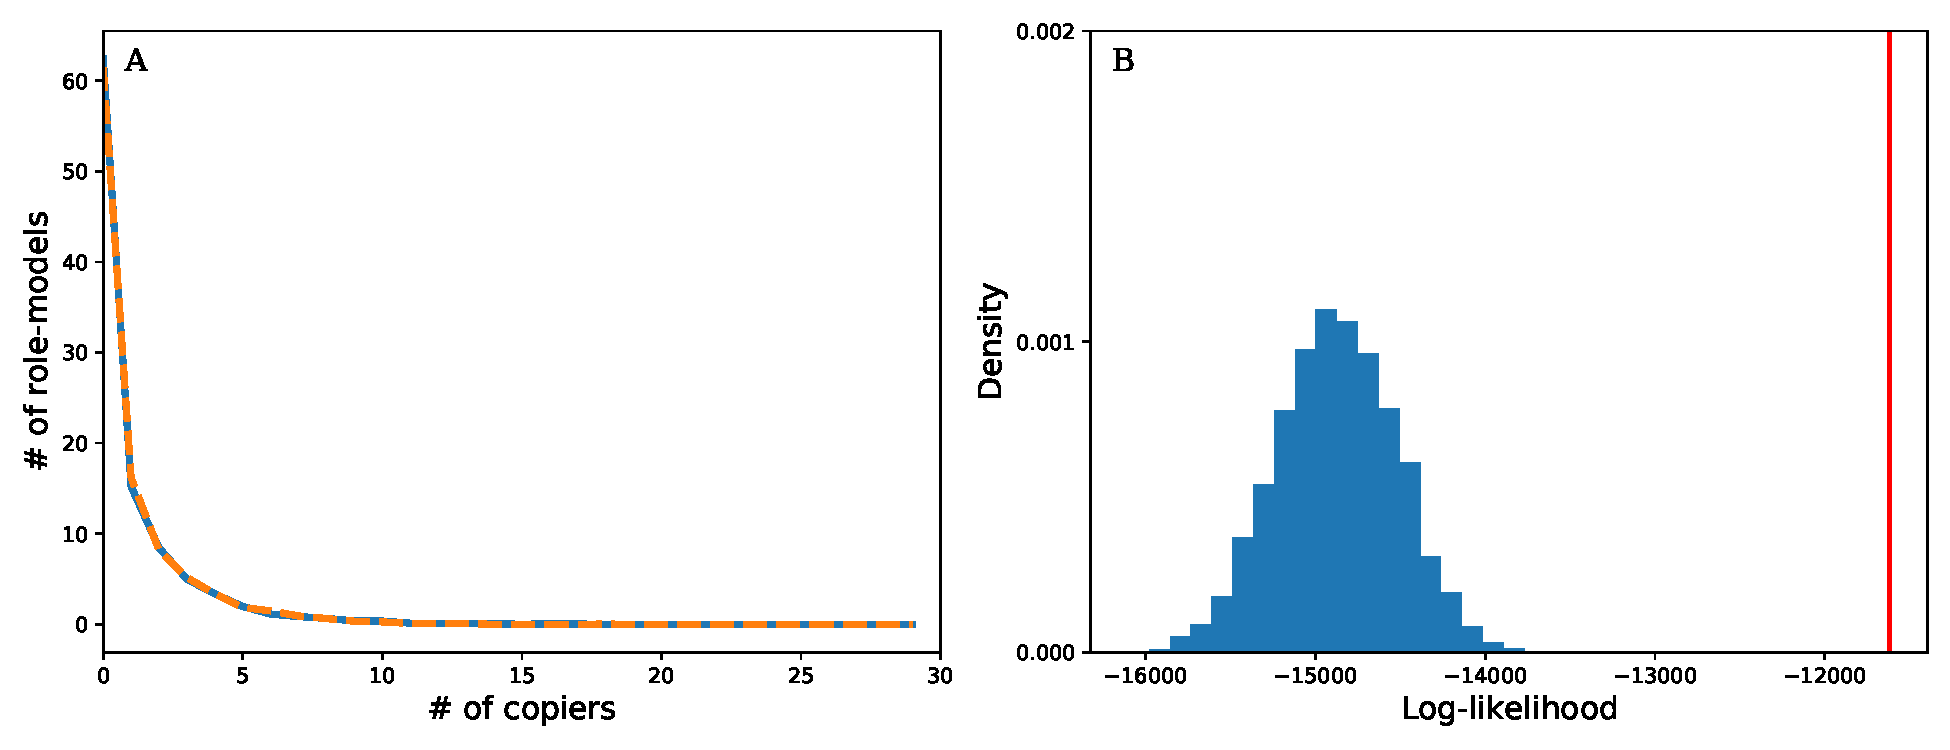
\includegraphics[width=\linewidth]{DM_validation.pdf}
  \caption{
  \textbf{Numerical validation of the DM approximation.}
  We performed computational simulations of the role-model choice process and compared them to the results of simulations using the DM distribution approximation.
  % TODO but what are these "results"?
  \textbf{(A)} The difference between the DM distribution (orange) and the empirical distribution of the simulations (blue) is very small. 
  \textbf{(B)} The log-likelihood of the DM distribution for results of the simulations (red vertical line) is much higher {than} the log-likelihood of permutations of simulations (blue histogram).
  Here, population size, $N=100$; number of simulations, $m=100$; phenotype values, $\hat{A}=1$, $A \sim N(0,1)$; success-bias weight, $\alpha=0.5$.
  No estimation error or bias is applied, and traits are estimated and copied perfectly.}	
  \label{fig:DM_validation}
\end{figure}


\begin{figure}[h]
    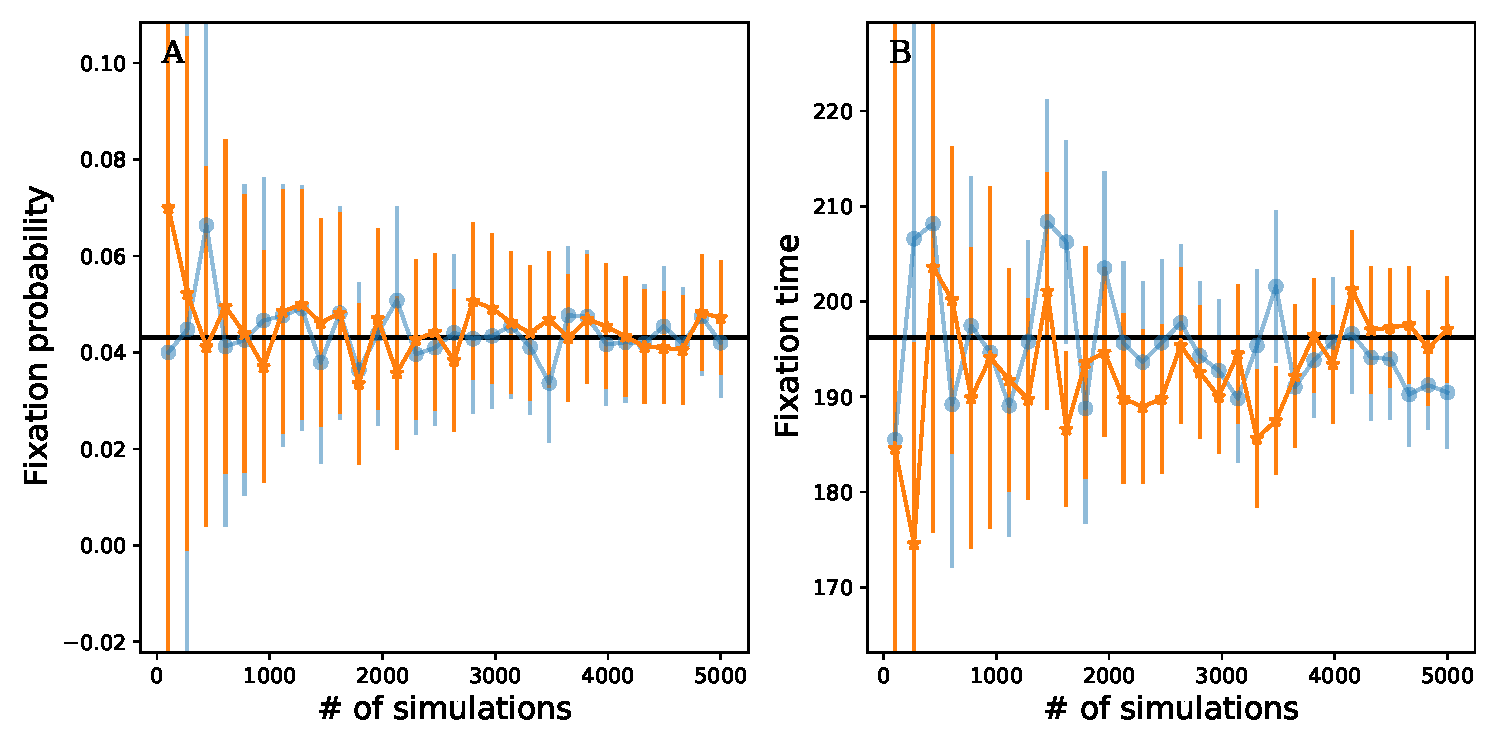
\includegraphics[width=\linewidth]{num_sims.pdf}
  \caption{
  \textbf{DM Approximation precision as function of number of simulations.}
  Our DM approximation (orange) agrees with stochastic simulation results (blue) when using 1,000 or more simulations.
  Both fluctuate around the analytic fixation probability approximation (black; \cref{eq:kimura_p}).
  Markers are averages across simulations, error bars are 95\% confidence intervals.
  Here, population size, $N=1000$; success-bias weight, $\alpha=0.5$; phenotype values, $\hat{A}=1$, $A=0.7$; success-bias value, $\beta(A)=0.956$.}	
  \label{fig:num_sims}
\end{figure}


\begin{figure}
    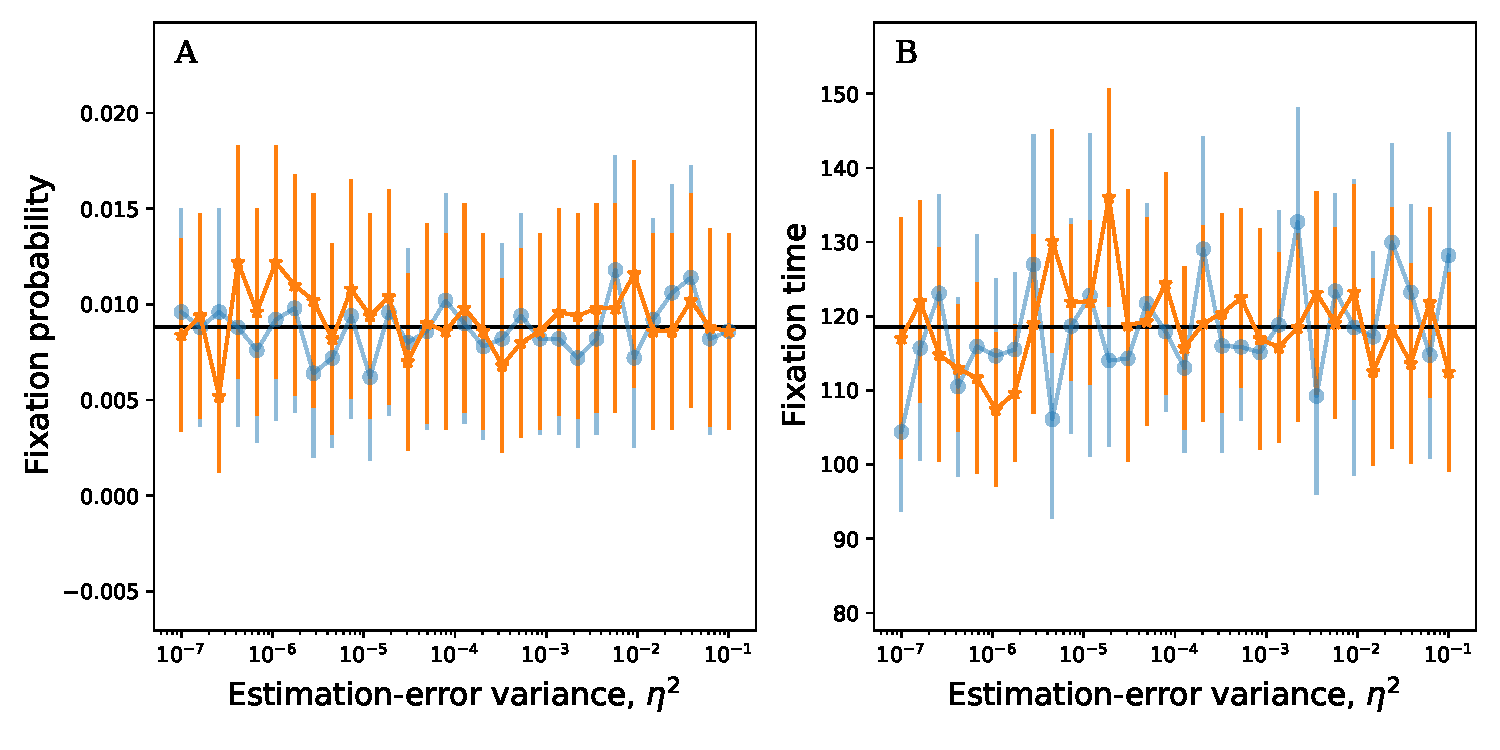
\includegraphics[width=\linewidth]{full_vs_dm_mutation.pdf}
  \caption{
  \textbf{Robustness of DM approximations to success estimation error.}
  Both the DM approximation (orange) and our approximation (black) agree with the stochastic simulations (blue), even with a high estimation error.
  Markers are averages across simulations, error bars are 95\% confidence intervals.
  5,000 simulations per data point; population size, $N=1000$; success-bias weight, $\alpha=0.1$; phenotype values, $\hat{A}=1$,$A=0.7$; bias strength parameter $J\sim N(1,\eta^2)$ where $\eta^2$ in on the x-axis.
  }	
  \label{fig:hetro_error}
\end{figure}


\begin{figure}
    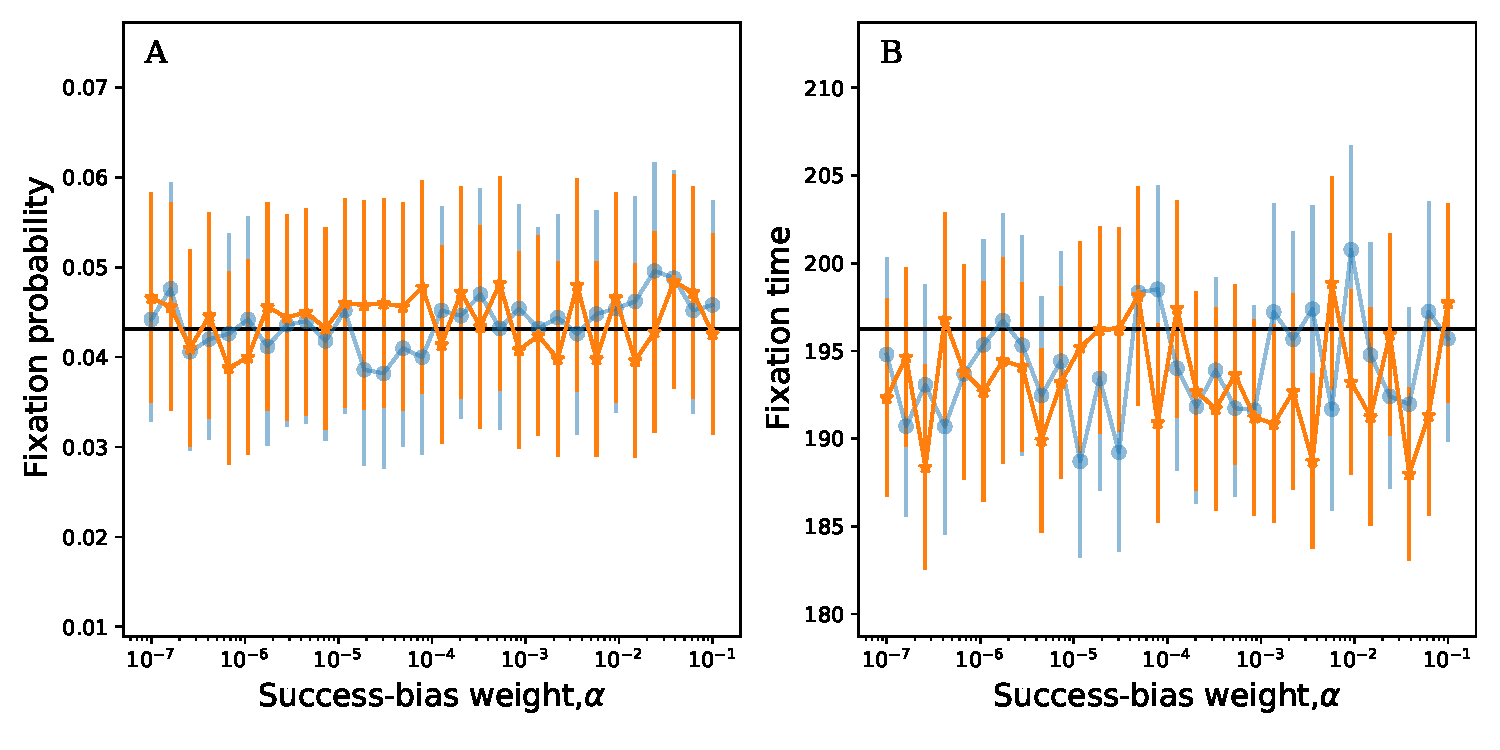
\includegraphics[width=\linewidth]{full_vs_dm_changing_alpha.pdf}
   \caption{\textbf{Robustness of DM approximations to variation in the bias weight $\alpha$.} 
   Both the DM approximation (orange) and Kimura's equation (black line) fit the stochastic simulations (blue) well even with a high variation in success bias weight. % TODO variation between... copiers? role-models?
   Markers for average across $5,000$ simulations, error bars are 95\% confidence intervals.
  Here, population size, $N=1000$; success bias weight normally distributed, $\alpha \sim N(0.5,\epsilon^2)$ where $e^{-7}\le \epsilon \le e^{-1}$; % TODO not clear to me: the x axes shows alpha, so how can alpha also be normally distributed ?
  phenotype values ,$\hat{A}=1$,$A=0.7$; success bias value, $\beta(A)=0.956$.}	
  \label{fig:hetro_alpha}
\end{figure}


\end{document}
